%%
% Copyright (c) 2017 - 2020, Pascal Wagler;
% Copyright (c) 2014 - 2020, John MacFarlane
%
% All rights reserved.
%
% Redistribution and use in source and binary forms, with or without
% modification, are permitted provided that the following conditions
% are met:
%
% - Redistributions of source code must retain the above copyright
% notice, this list of conditions and the following disclaimer.
%
% - Redistributions in binary form must reproduce the above copyright
% notice, this list of conditions and the following disclaimer in the
% documentation and/or other materials provided with the distribution.
%
% - Neither the name of John MacFarlane nor the names of other
% contributors may be used to endorse or promote products derived
% from this software without specific prior written permission.
%
% THIS SOFTWARE IS PROVIDED BY THE COPYRIGHT HOLDERS AND CONTRIBUTORS
% "AS IS" AND ANY EXPRESS OR IMPLIED WARRANTIES, INCLUDING, BUT NOT
% LIMITED TO, THE IMPLIED WARRANTIES OF MERCHANTABILITY AND FITNESS
% FOR A PARTICULAR PURPOSE ARE DISCLAIMED. IN NO EVENT SHALL THE
% COPYRIGHT OWNER OR CONTRIBUTORS BE LIABLE FOR ANY DIRECT, INDIRECT,
% INCIDENTAL, SPECIAL, EXEMPLARY, OR CONSEQUENTIAL DAMAGES (INCLUDING,
% BUT NOT LIMITED TO, PROCUREMENT OF SUBSTITUTE GOODS OR SERVICES;
% LOSS OF USE, DATA, OR PROFITS; OR BUSINESS INTERRUPTION) HOWEVER
% CAUSED AND ON ANY THEORY OF LIABILITY, WHETHER IN CONTRACT, STRICT
% LIABILITY, OR TORT (INCLUDING NEGLIGENCE OR OTHERWISE) ARISING IN
% ANY WAY OUT OF THE USE OF THIS SOFTWARE, EVEN IF ADVISED OF THE
% POSSIBILITY OF SUCH DAMAGE.
%%

%%
% This is the Eisvogel pandoc LaTeX template.
%
% For usage information and examples visit the official GitHub page:
% https://github.com/Wandmalfarbe/pandoc-latex-template
%%

\DeclareUnicodeCharacter{2212}{-}

% Options for packages loaded elsewhere
\PassOptionsToPackage{unicode}{hyperref}
\PassOptionsToPackage{hyphens}{url}
\PassOptionsToPackage{dvipsnames,svgnames*,x11names*,table}{xcolor}
%
\documentclass[
  12pt,
  a4paper,
,tablecaptionabove
]{scrartcl}
\usepackage{lmodern}
\usepackage{setspace}
\setstretch{1.2}
\usepackage{amssymb,amsmath}
\usepackage{ifxetex,ifluatex}
\ifnum 0\ifxetex 1\fi\ifluatex 1\fi=0 % if pdftex
  \usepackage[T1]{fontenc}
  \usepackage[utf8]{inputenc}
  \usepackage{textcomp} % provide euro and other symbols
\else % if luatex or xetex
  \usepackage{unicode-math}
  \defaultfontfeatures{Scale=MatchLowercase}
  \defaultfontfeatures[\rmfamily]{Ligatures=TeX,Scale=1}
\fi
% Use upquote if available, for straight quotes in verbatim environments
\IfFileExists{upquote.sty}{\usepackage{upquote}}{}
\IfFileExists{microtype.sty}{% use microtype if available
  \usepackage[]{microtype}
  \UseMicrotypeSet[protrusion]{basicmath} % disable protrusion for tt fonts
}{}
\makeatletter
\@ifundefined{KOMAClassName}{% if non-KOMA class
  \IfFileExists{parskip.sty}{%
    \usepackage{parskip}
  }{% else
    \setlength{\parindent}{0pt}
    \setlength{\parskip}{6pt plus 2pt minus 1pt}}
}{% if KOMA class
  \KOMAoptions{parskip=half}}
\makeatother
\usepackage{xcolor}
\definecolor{default-linkcolor}{HTML}{A50000}
\definecolor{default-filecolor}{HTML}{A50000}
\definecolor{default-citecolor}{HTML}{4077C0}
\definecolor{default-urlcolor}{HTML}{4077C0}
\IfFileExists{xurl.sty}{\usepackage{xurl}}{} % add URL line breaks if available
\IfFileExists{bookmark.sty}{\usepackage{bookmark}}{\usepackage{hyperref}}
\hypersetup{
  colorlinks=true,
  linkcolor=blue,
  filecolor=default-filecolor,
  citecolor=default-citecolor,
  urlcolor=default-urlcolor,
  breaklinks=true,
  pdfcreator={LaTeX via pandoc with the Eisvogel template}}
\urlstyle{same} % disable monospaced font for URLs
\usepackage[margin=1in]{geometry}
\usepackage{longtable,booktabs}
% Correct order of tables after \paragraph or \subparagraph
\usepackage{etoolbox}
\makeatletter
\patchcmd\longtable{\par}{\if@noskipsec\mbox{}\fi\par}{}{}
\makeatother
% Allow footnotes in longtable head/foot
\IfFileExists{footnotehyper.sty}{\usepackage{footnotehyper}}{\usepackage{footnote}}
\makesavenoteenv{longtable}
% add backlinks to footnote references, cf. https://tex.stackexchange.com/questions/302266/make-footnote-clickable-both-ways
\usepackage{footnotebackref}
\usepackage{graphicx}
\makeatletter
\def\maxwidth{\ifdim\Gin@nat@width>\linewidth\linewidth\else\Gin@nat@width\fi}
\def\maxheight{\ifdim\Gin@nat@height>\textheight\textheight\else\Gin@nat@height\fi}
\makeatother
% Scale images if necessary, so that they will not overflow the page
% margins by default, and it is still possible to overwrite the defaults
% using explicit options in \includegraphics[width, height, ...]{}
\setkeys{Gin}{width=\maxwidth,height=\maxheight,keepaspectratio}
\setlength{\emergencystretch}{3em}  % prevent overfull lines
\providecommand{\tightlist}{%
  \setlength{\itemsep}{0pt}\setlength{\parskip}{0pt}}
\setcounter{secnumdepth}{-\maxdimen} % remove section numbering
% Make \paragraph and \subparagraph free-standing
\ifx\paragraph\undefined\else
  \let\oldparagraph\paragraph
  \renewcommand{\paragraph}[1]{\oldparagraph{#1}\mbox{}}
\fi
\ifx\subparagraph\undefined\else
  \let\oldsubparagraph\subparagraph
  \renewcommand{\subparagraph}[1]{\oldsubparagraph{#1}\mbox{}}
\fi

% Make use of float-package and set default placement for figures to H.
% The option H means 'PUT IT HERE' (as  opposed to the standard h option which means 'You may put it here if you like').
\usepackage{float}
\floatplacement{figure}{H}

\usepackage{booktabs}
\usepackage{longtable}
\usepackage{array}
\usepackage{multirow}
\usepackage{wrapfig}
\usepackage{float}
\usepackage{colortbl}
\usepackage{pdflscape}
\usepackage{tabu}
\usepackage{threeparttable}
\usepackage{threeparttablex}
\usepackage[normalem]{ulem}
\usepackage{makecell}
\usepackage{xcolor}
\usepackage{xr}
\externaldocument{LMAms_SI}
\usepackage{lineno}
\linenumbers
\makeatletter
\makeatother
\makeatletter
\makeatother
\makeatletter
\@ifpackageloaded{caption}{}{\usepackage{caption}}
\AtBeginDocument{%
\ifdefined\contentsname
  \renewcommand*\contentsname{Table of contents}
\else
  \newcommand\contentsname{Table of contents}
\fi
\ifdefined\listfigurename
  \renewcommand*\listfigurename{List of Figures}
\else
  \newcommand\listfigurename{List of Figures}
\fi
\ifdefined\listtablename
  \renewcommand*\listtablename{List of Tables}
\else
  \newcommand\listtablename{List of Tables}
\fi
\ifdefined\figurename
  \renewcommand*\figurename{Fig.}
\else
  \newcommand\figurename{Fig.}
\fi
\ifdefined\tablename
  \renewcommand*\tablename{Table}
\else
  \newcommand\tablename{Table}
\fi
}
\@ifpackageloaded{float}{}{\usepackage{float}}
\floatstyle{ruled}
\@ifundefined{c@chapter}{\newfloat{codelisting}{h}{lop}}{\newfloat{codelisting}{h}{lop}[chapter]}
\floatname{codelisting}{Listing}
\newcommand*\listoflistings{\listof{codelisting}{List of Listings}}
\makeatother
\makeatletter
\@ifpackageloaded{caption}{}{\usepackage{caption}}
\@ifpackageloaded{subcaption}{}{\usepackage{subcaption}}
\makeatother
\makeatletter
\@ifpackageloaded{tcolorbox}{}{\usepackage[many]{tcolorbox}}
\makeatother
\makeatletter
\@ifundefined{shadecolor}{\definecolor{shadecolor}{rgb}{.97, .97, .97}}
\makeatother
\makeatletter
\makeatother

\newlength{\cslhangindent}
\setlength{\cslhangindent}{1.5em}
\newlength{\csllabelwidth}
\setlength{\csllabelwidth}{3em}
\newenvironment{CSLReferences}[2] % #1 hanging-ident, #2 entry spacing
 {% don't indent paragraphs
  \setlength{\parindent}{0pt}
  % turn on hanging indent if param 1 is 1
  \ifodd #1 \everypar{\setlength{\hangindent}{\cslhangindent}}\ignorespaces\fi
  % set entry spacing
  \ifnum #2 > 0
  \setlength{\parskip}{#2\baselineskip}
  \fi
 }%
 {}
\usepackage{calc}
\newcommand{\CSLBlock}[1]{#1\hfill\break}
\newcommand{\CSLLeftMargin}[1]{\parbox[t]{\csllabelwidth}{#1}}
\newcommand{\CSLRightInline}[1]{\parbox[t]{\linewidth - \csllabelwidth}{#1}\break}
\newcommand{\CSLIndent}[1]{\hspace{\cslhangindent}#1}

\date{}


%%
%% added
%%

%
% language specification
%
% If no language is specified, use English as the default main document language.
%

\ifnum 0\ifxetex 1\fi\ifluatex 1\fi=0 % if pdftex
  \usepackage[shorthands=off,main=english]{babel}
\else
    % Workaround for bug in Polyglossia that breaks `\familydefault` when `\setmainlanguage` is used.
  % See https://github.com/Wandmalfarbe/pandoc-latex-template/issues/8
  % See https://github.com/reutenauer/polyglossia/issues/186
  % See https://github.com/reutenauer/polyglossia/issues/127
  \renewcommand*\familydefault{\sfdefault}
    % load polyglossia as late as possible as it *could* call bidi if RTL lang (e.g. Hebrew or Arabic)
  \usepackage{polyglossia}
  \setmainlanguage[]{english}
\fi



%
% for the background color of the title page
%

%
% break urls
%
\PassOptionsToPackage{hyphens}{url}

%
% When using babel or polyglossia with biblatex, loading csquotes is recommended
% to ensure that quoted texts are typeset according to the rules of your main language.
%
\usepackage{csquotes}

%
% captions
%
%\definecolor{caption-color}{HTML}{777777}
\definecolor{caption-color}{HTML}{37474F}
%\usepackage[font={stretch=1.2}, textfont={color=caption-color}, position=top, skip=4mm, labelfont=bf, singlelinecheck=false, justification=raggedright]{caption}
\usepackage[font={stretch=1}, textfont={color=caption-color}, position=top, skip=2mm, labelfont=bf, singlelinecheck=false, justification=raggedright]{caption}
\setcapindent{0em}

%
% blockquote
%
\definecolor{blockquote-border}{RGB}{221,221,221}
\definecolor{blockquote-text}{RGB}{119,119,119}
\usepackage{mdframed}
\newmdenv[rightline=false,bottomline=false,topline=false,linewidth=3pt,linecolor=blockquote-border,skipabove=\parskip]{customblockquote}
\renewenvironment{quote}{\begin{customblockquote}\list{}{\rightmargin=0em\leftmargin=0em}%
\item\relax\color{blockquote-text}\ignorespaces}{\unskip\unskip\endlist\end{customblockquote}}

%
% Source Sans Pro as the de­fault font fam­ily
% Source Code Pro for monospace text
%
% 'default' option sets the default
% font family to Source Sans Pro, not \sfdefault.
%
\ifnum 0\ifxetex 1\fi\ifluatex 1\fi=0 % if pdftex
    \usepackage[default]{sourcesanspro}
  \usepackage{sourcecodepro}
  %\usepackage{}
  \else % if not pdftex
    \usepackage[default]{sourcesanspro}
  \usepackage{sourcecodepro}
  %\usepackage{}

  % XeLaTeX specific adjustments for straight quotes: https://tex.stackexchange.com/a/354887
  % This issue is already fixed (see https://github.com/silkeh/latex-sourcecodepro/pull/5) but the
  % fix is still unreleased.
  % TODO: Remove this workaround when the new version of sourcecodepro is released on CTAN.
  \ifxetex
    \makeatletter
    \defaultfontfeatures[\ttfamily]
      { Numbers   = \sourcecodepro@figurestyle,
        Scale     = \SourceCodePro@scale,
        Extension = .otf }
    \setmonofont
      [ UprightFont    = *-\sourcecodepro@regstyle,
        ItalicFont     = *-\sourcecodepro@regstyle It,
        BoldFont       = *-\sourcecodepro@boldstyle,
        BoldItalicFont = *-\sourcecodepro@boldstyle It ]
      {SourceCodePro}
    \makeatother
  \fi
  \fi

%
% heading color
%
\definecolor{heading-color}{RGB}{40,40,40}
\addtokomafont{section}{\color{heading-color}}
% When using the classes report, scrreprt, book,
% scrbook or memoir, uncomment the following line.
%\addtokomafont{chapter}{\color{heading-color}}

%
% variables for title and author
%
\usepackage{titling}
\title{}
\author{}

%
% tables
%

\definecolor{table-row-color}{HTML}{F5F5F5}
\definecolor{table-rule-color}{HTML}{999999}

%\arrayrulecolor{black!40}
\arrayrulecolor{table-rule-color}     % color of \toprule, \midrule, \bottomrule
\setlength\heavyrulewidth{0.3ex}      % thickness of \toprule, \bottomrule
\renewcommand{\arraystretch}{1.3}     % spacing (padding)


%
% remove paragraph indention
%
\setlength{\parindent}{0pt}
\setlength{\parskip}{6pt plus 2pt minus 1pt}
\setlength{\emergencystretch}{3em}  % prevent overfull lines

%
%
% Listings
%
%


%
% header and footer
%
\usepackage{fancyhdr}

\fancypagestyle{eisvogel-header-footer}{
  \fancyhead{}
  \fancyfoot{}
  \lhead[]{}
  \chead[]{}
  \rhead[]{}
  %\lfoot[\thepage]{}
  \cfoot[]{}
  \cfoot[]{\thepage}
  \renewcommand{\headrulewidth}{0.0pt}
 % \renewcommand{\footrulewidth}{0.0pt}
 % \renewcommand{\headrulewidth}{0.4pt}
 % \renewcommand{\footrulewidth}{0.4pt}
}
\pagestyle{eisvogel-header-footer}

%%
%% end added
%%

\begin{document}

%%
%% begin titlepage
%%

%%
%% end titlepage
%%



\ifdefined\Shaded\renewenvironment{Shaded}{\begin{tcolorbox}[boxrule=0pt, enhanced, frame hidden, sharp corners, interior hidden, borderline west={3pt}{0pt}{shadecolor}, breakable]}{\end{tcolorbox}}\fi

\textbf{Running title}: Metabolic and structural leaf mass

\textbf{Decomposing leaf mass into metabolic and structural components
explains divergent patterns of trait variation within and among plant
species}

Masatoshi Katabuchi\textsuperscript{1,2,6}, Kaoru
Kitajima\textsuperscript{2,3,4}, S. Joseph Wright\textsuperscript{4},
Sunshine A. Van Bael\textsuperscript{4,5}, Jeanne L. D.
Osnas\textsuperscript{2} and Jeremy W. Lichstein\textsuperscript{2}

\textsuperscript{1} Xishuangbanna Tropical Botanical Garden, Chinese
Academy of Sciences, Menglun, Yunnan 666303 China

\textsuperscript{2} Department of Biology, University of Florida,
Gainesville, FL 32611, USA

\textsuperscript{3} Graduate School of Agriculture, Kyoto University,
Kitashirakawa Oiwake-Cho, Kyoto 606-8502 Japan

\textsuperscript{4} Smithsonian Tropical Research Institute, 9100 Panama
City Pl., Washington, DC 20521

\textsuperscript{5} Department of Ecology and Evolutionary Biology,
Tulane University, New Orleans, LA 70118 USA

\textsuperscript{6} \textbf{Corresponding Author}: E-mail:
mattocci27@gmail.com

\begin{itemize}
\item
  Across the global flora, photosynthetic and metabolic rates depend
  more strongly on leaf area than leaf mass. In contrast, intraspecific
  variation in these rates is strongly mass-dependent. These contrasting
  patterns suggest that the causes of variation in leaf mass per area
  (LMA) may be fundamentally different within vs.~among species.
\item
  We developed statistical modeling framework to decompose LMA into two
  conceptual components -- metabolic LMAm (which determines
  photosynthetic capacity and dark respiration) and structural LMAs
  (which determines leaf toughness and potential leaf lifespan) - using
  leaf trait data from tropical forest sites in Panama and a global
  leaf-trait database.
\item
  Decomposing LMA into LMAm and LMAs provides improved predictions of
  leaf trait variation (photosynthesis, respiration, and lifespan). We
  show that strong area-dependence of metabolic traits across species
  can result from multiple of factors, including high LMAs variance
  and/or a slow increase in photosynthetic capacity with increasing
  LMAm. In contrast, strong mass-dependence of metabolic traits within
  species across light levels results from LMAm increasing from sun to
  shade. LMAm and LMAs were nearly independent of each other in both
  global and Panama datasets.
\item
  Our results suggest that leaf functional variation is
  multi-dimensional and that biogeochemical models should treat
  metabolic and structural leaf components separately.
\end{itemize}

\hypertarget{introduction}{%
\section{Introduction}\label{introduction}}

Leaf functional traits play an important role in ecological and
physiological tradeoffs (\protect\hyperlink{ref-Onoda2017}{Onoda et al.,
2017}; \protect\hyperlink{ref-Reich2014}{Reich, 2014};
\protect\hyperlink{ref-Wright2004a}{I. J. Wright et al., 2004}) and in
carbon and nutrient cycling (e.g.,
\protect\hyperlink{ref-Huntingford2017}{Huntingford et al., 2017};
\protect\hyperlink{ref-Tcherkez2017}{Tcherkez et al., 2017}). Thus,
understanding the causes and consequences of leaf trait variation is an
important goal in ecology, plant physiology, and biogeochemistry
(\protect\hyperlink{ref-Bonan2002}{Bonan et al., 2002};
\protect\hyperlink{ref-Poorter2009}{Poorter et al., 2009}). Different
leaf assemblages exhibit markedly different patterns of trait variation.
For example, across global species, whole-leaf values of traits related
to photosynthesis and metabolism (e.g., the photosynthetic capacity,
respiration rate, or nutrient content of entire leaves) tend to increase
more strongly with leaf area than leaf mass (Osnas et al.
(\protect\hyperlink{ref-Osnas2013}{2013})), whereas the opposite pattern
(strong mass-dependence of these same traits) is observed within species
across canopy light gradients (\protect\hyperlink{ref-Osada2001}{Osada
et al., 2001}; \protect\hyperlink{ref-Osnas2018}{Osnas et al., 2018}).
Functional groups (e.g., deciduous vs.~evergreen angiosperms) also
differ from each other in terms of how photosynthetic and metabolic
traits variation depend on leaf mass and area
(\protect\hyperlink{ref-Osnas2018}{Osnas et al., 2018}). These divergent
patterns suggest the presence of multiple drivers of trait variation.

Strong interspecific correlations among leaf mass per area (LMA), leaf
lifespan (LL), and mass-normalized leaf traits related to photosynthesis
and metabolism (hereafter, `metabolic traits') have been interpreted as
evidence for a single dominant axis of leaf functional variation
(\protect\hyperlink{ref-Wright2004a}{I. J. Wright et al., 2004}).
However, the interpretation of these strong correlations, which result
from mass-normalization of area-dependent traits
(\protect\hyperlink{ref-Lloyd2013}{Lloyd et al., 2013};
\protect\hyperlink{ref-Osnas2013}{Osnas et al., 2013}), is
controversial. On the one hand, mass-normalization has been justified
based on economic principles alone
(\protect\hyperlink{ref-Westoby2013}{Westoby et al., 2013}), because
leaf mass provides a simple index of investment that underlies the leaf
economics spectrum (LES), ranging from cheap, low-LMA leaves with a fast
rate of return per-unit investment to expensive, high-LMA leaves with a
slow rate of return (\protect\hyperlink{ref-Wright2004a}{I. J. Wright et
al., 2004}). On the other hand, because the lifetime return on
investment depends on LL (\protect\hyperlink{ref-Falster2012}{Falster et
al., 2012}; \protect\hyperlink{ref-Westoby2000}{Westoby et al., 2000}),
and normalizing traits by their annualized construction costs (or
mass/LL) should be used as a normalizer in leaf economics analyses
(\protect\hyperlink{ref-Osnas2013}{Osnas et al., 2013}). In global
analyses, normalizing leaf traits by mass/LL yields similarly weak
correlations as area-normalization, because leaf area is roughly
proportional to mass/LL across global species
(\protect\hyperlink{ref-Osnas2013}{Osnas et al., 2013}). Area-dependence
of metabolic traits and the inconsistent correlation strengths obtained
from different normalizers (\protect\hyperlink{ref-Lloyd2013}{Lloyd et
al., 2013}; \protect\hyperlink{ref-Osnas2013}{Osnas et al., 2013}) do
not invalidate mass-normalization or the LES
(\protect\hyperlink{ref-Westoby2013}{Westoby et al., 2013}) These
considerations do, however, lead us to question the evidence for a
single dominant axis of leaf functional diversity, which has important
implications for how trait variation is represented in ecosystem models
(\protect\hyperlink{ref-Bonan2002}{Bonan et al., 2002};
\protect\hyperlink{ref-Sakschewski2016}{Sakschewski et al., 2016}).

To understand why the same data can be interpreted as either supporting
or opposing the existence of a single dominant axis of leaf trait
variation, consider the conceptual model proposed by Osnas et al.
(\protect\hyperlink{ref-Osnas2018}{2018}), in which LMA is comprised of
two additive components: photosynthetic LMA (LMAm) -- the mass per area
of chloroplasts and other metabolically active leaf components that
contribute directly to photosynthesis and respiration -- and structural
LMA (LMAs) -- the mass per area of structural leaf components that
contribute to toughness and durability
(\protect\hyperlink{ref-Kitajima2016}{Kitajima et al., 2016},
\protect\hyperlink{ref-Kitajima2012}{2012};
\protect\hyperlink{ref-Onoda2017}{Onoda et al., 2017}). Suppose these
two LMA components are independent axes of functional variation, so that
LMAm and LMAs are uncorrelated across species (Fig.~\ref{fig-Hplt}a).
These two independent axes can be translated into either a
two-dimensional trait space (if metabolic traits are area-normalized;
Fig.~\ref{fig-Hplt}b) or a one-dimensional trait space (if metabolic
traits are mass-normalized; Fig.~\ref{fig-Hplt}c). While both
Fig.~\ref{fig-Hplt}b and Fig.~\ref{fig-Hplt}c are both `correct'
representations of the same data, they lead to different perceptions
about the dimensionality of leaf functional variation. If LMAm, LMAs,
and/or other axes are largely independent and have distinct functional
consequences, then it would not be possible to accurately represent
functional variation with a single axis.

The hypothetical example in Fig.~\ref{fig-Hplt} shows how
mass-normalization can, in principle, make a two-dimensional trait space
appear one-dimensional, but the dimensionality of functional variation
in real leaf assemblages remains an open question. One way to better
understand the dimensionality of leaf trait variation is to compare
models with different numbers of dimensions, and to ask if models with
multiple dimensions provide improved statistical fits and conceptual
insights compared to a single axis. For example, the two-dimensional
`LMAm + LMAs' model proposed by Osnas et al.
(\protect\hyperlink{ref-Osnas2018}{2018}) could be compared to a
one-dimensional LMA model in terms of their capacities to explain
variation in other traits. However, implementing the `LMAm + LMAs' model
is challenging, because although certain leaf mass components can be
neatly classified as `metabolic' or `structural'
(\protect\hyperlink{ref-Osnas2018}{Osnas et al., 2018};
\protect\hyperlink{ref-Poorter2009}{Poorter et al., 2009}), other leaf
mass components cannot. For example, thick cell walls contribute to
structural toughness (\protect\hyperlink{ref-Onoda2015}{Onoda et al.,
2015}), but at least some cell wall mass is required for the
biomechanical support that enables photosynthesis. Thus, partitioning
LMA into different functional components requires novel empirical or
modeling approaches.

In this paper, we present a statistical modeling framework to partition
LMA into metabolic and structural components: LMAm and LMAs. We develop
and test this two-dimensional model using leaf trait data from two
tropical forest sites (sun and shade leaves from wet and dry sites in
Panama) and the GLOPNET global leaf traits database
(\protect\hyperlink{ref-Wright2004a}{I. J. Wright et al., 2004}). We use
the model to address the following questions: (1) Are measured leaf
traits (including photosynthetic capacity, dark respiration rate, LL,
and concentrations of nutrients and cellulose) better predicted by a
one-dimensional (total LMA) or two-dimensional (LMAm-LMAs) model? (2)
What are the relative contributions of LMAm and LMAs to total LMA
variance in different leaf assemblages (Panama sun leaves, Panama shade
leaves, and the global flora)? (3) Do LMAm and LMAs differ between
evergreen and deciduous species, and between sun and shade leaves? If
so, how? and (4) How do the answers to the preceding questions inform
our understanding of empirical patterns of trait variation (e.g.,
relationships among measured leaf traits)?

\hypertarget{material-and-methods}{%
\section{Material and Methods}\label{material-and-methods}}

\hypertarget{overview}{%
\subsection{Overview}\label{overview}}

We considered multiple approaches to modeling datasets that include
observations of leaf mass per area (LMA), leaf lifespan (LL), net
photosynthetic capacity (\emph{A}), and dark respiration rate
(\emph{R}). These traits comprise four of the six traits in the global
leaf economics spectrum (LES) analysis of I. J. Wright et al.
(\protect\hyperlink{ref-Wright2004a}{2004}). For simplicity, we did not
include the other two LES traits -- leaf nitrogen (\emph{N}) and
phosphorus (\emph{P}) concentrations -- in our modeling framework.
Instead, we reserved observations of leaf \emph{N} and \emph{P}
concentrations (and cellulose content, when available) for independent
model tests. We considered a simple one-dimensional model that predicts
LL, \emph{A}, and \emph{R} from LMA alone, as well as two-dimensional
models that predict LL, \emph{A}, and \emph{R} from two additive LMA
components: structural and metabolic and structural leaf mass per area
(LMAm and LMAs, respectively). We formulate the models in terms of
area-normalized \emph{A} and \emph{R} (\emph{A}\textsubscript{area} and
\emph{R}\textsubscript{area}, respectively), as these trait forms share
the same denominator as LMA and its components.

To implement the two-dimensional models, we developed a statistical
modeling framework to partition LMA into additive LMAm and LMAs
components. We fit the models to two datasets: the GLOPNET global leaf
traits dataset (\protect\hyperlink{ref-Wright2004a}{I. J. Wright et al.,
2004}), which primarily represents interspecific variation; and the
Panama dataset described by Osnas et al.
(\protect\hyperlink{ref-Osnas2018}{2018}), which includes traits for
both sun and shade leaves at wet and dry tropical forest sites. Because
LMAm and LMAs are modeled (rather than observed), the two-dimensional
models require one parameter per analysis unit (a species in GLOPNET or
a species \(\times\) canopy-position in the Panama dataset) to partition
observed LMA into LMAm and LMAs. Given the large number of parameters in
these models, we performed tests with randomized data to evaluate if our
two-dimensional models were prone to overfitting, which could lead to
spurious conclusions. These tests suggested that our two-dimensional
modeling approach revealed meaningful patterns in the observed trait
data.

\hypertarget{modeling-leaf-lifespan-photosynthetic-capacity-and-dark-respiration-rate}{%
\subsection{Modeling leaf lifespan, photosynthetic capacity, and dark
respiration
rate}\label{modeling-leaf-lifespan-photosynthetic-capacity-and-dark-respiration-rate}}

We considered five types of models, ranging from simple models with LMA
as the sole predictor, to more complex models in which LMA was
partitioned into LMAm and LMAs. In all models, the unit of analysis is a
`leaf sample', defined as a species in the GLOPNET dataset or a species
\(\times\) canopy position in the Panama dataset (the datasets are
described below).

First, we considered a simple set of models with LMA as the sole
predictor for \emph{A}\textsubscript{area},
\emph{R}\textsubscript{area}, and LL according to power-law
relationships.

Next, we considered models in which LMA is partitioned into additive
metabolic and structural components for leaf sample \emph{i}:

\begin{equation}\protect\hypertarget{eq-LMA}{}{
\begin{aligned}
  &\mathrm{LMA}_{i} =\mathrm{LMAm}_{i} + \mathrm{LMAs}_{i} \\
  &\mathrm{LMAm}_{i} = f_{i} \mathrm{LMA}_{i} \\
  &\mathrm{LMAs}_{i} = (1 - f_{i})  \mathrm{LMA}_{i}
\end{aligned}
}\label{eq-LMA}\end{equation}

where the \emph{f\textsubscript{i}} values -- the fractions of LMA
comprised of LMAm for each sample \emph{i} -- are estimated as latent
variables in our modeling framework (see details below). We assumed that
the observed values of \emph{A}\textsubscript{area},
\emph{R}\textsubscript{area} and LL were related to the unobserved
values LMAm and LMAs according to multivariate power-laws:

\begin{align}
& \mathrm{E}[A_{\mathrm{area} \, i}]
= \alpha_0\mathrm{LMAm}_{i}^{\alpha_m}\mathrm{LMAs}_i^{\alpha_s}  =  \alpha_0 (f_i \mathrm{LMA}_{i})^{\alpha_m} \bigl\{(1-f_i) \mathrm{LMA}_{i}\bigr\}^{\alpha_s} \label{eq:Aarea} \\
& \mathrm{E}[R_{\mathrm{area} \, i}]
= \gamma_0\mathrm{LMAm}_{i}^{\gamma_p} \mathrm{LMAs}_{i}^{\gamma_s}
= \gamma_0 (f_i \mathrm{LMA}_{i})^{\gamma_p} \bigl\{(1-f_i)\mathrm{LMA}_{i}\bigr\}^{\gamma_s} \label{eq:Rarea} \\
& \mathrm{E}[\mathrm{LL}_i] = \beta_0\mathrm{LMAm}_{i}^{\beta_m} \mathrm{LMAs}_{i}^{\beta_s}  = \beta_0 (f_i \mathrm{LMA}_{i})^{\beta_m} \bigl\{(1-f_i) \mathrm{LMA}_{i}\bigr\}^{\beta_s} \label{eq:LL_pot} \tag{4a}  \\
& \mathrm{E[LL}_i] = \beta_0\mathrm{LMAm}_{i}^{\beta_m} \mathrm{LMAs}_{i}^{\beta_s} \mathrm{exp}(\theta \mathrm{Light}_i)  \stepcounter{equation} \label{eq:LL_opt} \tag{4b}
\end{align}

where E{[}\(\cdot\){]} indicates expected value; the \(\alpha\),
\(\beta\), and \(\gamma\) terms are fitted parameters; and the
logarithms of \emph{A}\textsubscript{area}, LL, and
\emph{R}\textsubscript{area} are assumed to have a multivariate normal
distribution (Appendix S1). In preliminary analyses, we also considered
alternative (non-power-law) forms, but none of these performed better
than the power-law forms and are not discussed further.

To ensure that the model was identifiable, we imposed two broad
assumptions: (i) \emph{A}\textsubscript{area} depends more strongly on
metabolic leaf mass (LMAm: parameter \(\alpha_m\) in \ref{eq:Aarea})
than structural leaf mass (LMAs: parameter \(\alpha_s\)), and (ii) LL
depends more strongly on LMAs (\(\beta_s\) in
Eqs.\ref{eq:LL_pot}-\ref{eq:LL_opt}) than LMAm (\(\beta_m\)). The first
assumption was implemented in different model versions either by setting
\(\alpha_s\) = 0 or by imposing the constraint \(\alpha_m\)
\textgreater{} \(\alpha_s\). Similarly, the second assumption was
implemented either by setting \(\beta_m\) = 0 or by imposing the
constraint \(\beta_s\) \textgreater{} \(\beta_m\). The weaker form of
these assumptions (\(\alpha_m\) \textgreater{} \(\alpha_s\) and
\(\beta_s\) \textgreater{} \(\beta_m\)) is primarily a labeling
constraint and only weakly constrains the possible biological model
outcomes by excluding the possibility that a single LMA component could
be the primary determinant of both \emph{A}\textsubscript{area} and LL.
The stronger form of the assumptions (\(\alpha_s\) = 0 and \(\beta_m\) =
0) leads to a more parsimonious model (fewer parameters). We considered
different combinations of the strong and weak forms of the assumptions
for \emph{A}\textsubscript{area} (\(\alpha_m\) and \(\alpha_s\)) and LL
(\(\beta_s\) and \(\beta_m\)) using cross-validation (see details
below). We did not impose any constraints on
\emph{R}\textsubscript{area} (\(\gamma_s\) and \(\gamma_m\)).

We also considered models in which LMAs in Eqs.
\ref{eq:LL_pot}-\ref{eq:LL_opt} was replaced by leaf structural density
(LMAs/LT, where LT is leaf thickness), which is based on the observation
that cellulose density is a good predictor for LL in some species
assemblages (\protect\hyperlink{ref-Kitajima2013}{Kitajima et al.,
2013}, \protect\hyperlink{ref-Kitajima2012}{2012}). These models with
LMAs/LT yielded qualitatively similar results as those based on LMAs,
but did not perform as well in the model evaluation (see below).
Therefore, we only present results from the models with LMAs.

Finally, we considered a functional form that accounts for the effects
of light availability on LL. This light-dependent model is motivated by
optimal LL theory, which predicts decreasing LL with increasing light
availability (\protect\hyperlink{ref-Kikuzawa1991}{Kikuzawa, 1991}), and
also by the often-observed `LMA counter-gradient', whereby LL and LMA
positively covary across species but negatively covary within species
across light gradients (\protect\hyperlink{ref-Lusk2008}{Lusk et al.,
2008}; \protect\hyperlink{ref-Osnas2018}{Osnas et al., 2018};
\protect\hyperlink{ref-Russo2016}{Russo \& Kitajima, 2016}).
Mechanistically modeling how light affects LL via leaf carbon balance
(\protect\hyperlink{ref-Xu2017}{Xu et al., 2017}) is beyond the scope of
our study. Instead, we introduced light effects in a simple way by
modifying Eq. \ref{eq:LL_pot} to Eq. \ref{eq:LL_opt} where the dummy
variable Light\textsubscript{\emph{i}} is set to 1 for sun leaves and 0
for shade leaves, and exp(\(\theta\)) is the sun:shade LL ratio.

\hypertarget{datasets}{%
\subsection{Datasets}\label{datasets}}

We fit the models described above using observations of LMA (g
m\textsuperscript{-2}), \emph{A}\textsubscript{area} (mol
s\textsuperscript{-1} m\textsuperscript{-2}),
\emph{R}\textsubscript{area} (mol s\textsuperscript{-1}
m\textsuperscript{-2}) and LL (months) from the GLOPNET global leaf
traits database (\protect\hyperlink{ref-Wright2004a}{I. J. Wright et
al., 2004}) and from two tropical forest sites in Panama: Monumental
Natural Metropolitano (MNM, ``dry site'') and Bosque Protector San
Lorenzo (SL, ``wet site''). The GLOPNET data primarily represents
interspecific variation (the dataset reports 2,548 species \(\times\)
site combinations, with 2,021 unique species and only 350 species
occurring at more than one site) and only reports data for sun leaves if
data for both sun and shade leaves are available
(\protect\hyperlink{ref-Wright2004a}{I. J. Wright et al., 2004}). In
contrast, the Panama dataset represents both inter- and intraspecific
variation, including leaves sampled at two canopy positions (``sun'':
full sun at the top of the canopy; and ``shade'': well shaded, sampled
within 2 m of the forest floor) from trees within reach of canopy
cranes. The dry MNM site is a semi-deciduous coastal Pacific forest with
a 5-month dry season from December-April and 1740 mm of annual rainfall
(\protect\hyperlink{ref-Wright2003}{S. J. Wright et al., 2003}). The MNM
crane is 40 m tall with a 51 m long boom. The wet SL site is an
evergreen Caribbean coastal forest with 3100 mm of annual rainfall
(\protect\hyperlink{ref-Wright2003}{S. J. Wright et al., 2003}). The SL
crane is 52 m tall with a 54 m long boom. Additional details of the
Panama dataset are described in Osnas et al.
(\protect\hyperlink{ref-Osnas2018}{2018}).

We restricted our analysis to database records for which all four traits
(LMA, \emph{A}\textsubscript{area}, \emph{R}\textsubscript{area}, and
LL; each typically averaged over multiple leaves) were available. Each
database record corresponds to an analysis unit (or `leaf sample') as
described above; i.e., a species in GLOPNET, or a species \(\times\)
canopy position in the Panama dataset. After excluding database records
that lacked one or more of the four traits, 198 samples for 198 unique
species were available for GLOPNET, and 130 samples for 104 unique
species were available for Panama (dry and wet sites combined; 26
species sampled in both sun and shade; no species with all four traits
available at both sites). In addition to LMA,
\emph{A}\textsubscript{area}, \emph{R}\textsubscript{area}, and LL, the
model based on structural leaf density also requires observations of
leaf thickness, which was not available in GLOPNET but was available for
106/130 Panama samples. Both the GLOPNET and Panama datasets include
additional traits that we used to interpret model results, but which
were not used to fit models. These traits include nitrogen and
phosphorus content per leaf unit area (\emph{N}\textsubscript{area} and
\emph{P}\textsubscript{area}; g m\textsuperscript{-2}) and leaf
habit(deciduous or evergreen), and cellulose content per unit area
(\emph{CL}\textsubscript{area}; g m\textsuperscript{-2}) in the Panama
dataset.

\hypertarget{model-estimation-and-evaluation}{%
\subsection{Model estimation and
evaluation}\label{model-estimation-and-evaluation}}

We modeled \emph{A}\textsubscript{area} and \emph{R}\textsubscript{area}
using Eqs. \ref{eq:Aarea} and \ref{eq:Rarea}, respectively, for both
GLOPNET and Panama. To model LL for GLOPNET, we used Eq. \ref{eq:LL_pot}
(no light effects), because GLOPNET does not report canopy position (and
prioritizes data for sun leaves, as described above). To model LL for
Panama, we used Eq. \ref{eq:LL_opt} (light effects model), which was
motivated by the negative intraspecific LL-LMA relationship observed in
Panama (\protect\hyperlink{ref-Osnas2018}{Osnas et al., 2018};
\protect\hyperlink{ref-Xu2017}{Xu et al., 2017}) and elsewhere
(\protect\hyperlink{ref-Lusk2008}{Lusk et al., 2008};
\protect\hyperlink{ref-Russo2016}{Russo \& Kitajima, 2016}).

Posterior distributions of all parameters were estimated using the
Hamiltonian Monte Carlo algorithm (HMC) implemented in Stan
(\protect\hyperlink{ref-Carpenter2017}{Carpenter et al., 2017}). We used
non-informative or weakly informative prior distributions
(\protect\hyperlink{ref-Lemoine2019}{Lemoine, 2019}). Prior
distributions for the latent variables \emph{f\textsubscript{i}} (which
are used to partition LMA into LMAm and LMAs according to
Eq.~\ref{eq-LMA} were non-informative uniform(0, 1) distributions,
(i.e., LMA was partitioned based on patterns in the data). See Appendix
S1 for more detail. The Stan code use to fit models is available from
Github at: \url{https://github.com/mattocci27/LMAms}. Convergence of the
posterior distribution was assessed with the Gelman-Rubin statistic with
a convergence threshold of 1.05 for all parameters
(\protect\hyperlink{ref-Gelman2013}{Gelman et al., 2013}).

Because our two-dimensional (LMAm-LMAs) modeling approach includes many
parameters (one latent variable \emph{f\textsubscript{i}} to partition
LMA into LMAm and LMAs for each leaf sample), we implemented tests with
randomized data to assess potential overfitting. We generated 10
different randomized datasets by randomizing all trait values (LMA,
\emph{A}\textsubscript{area}, \emph{R}\textsubscript{area} and LL)
across species. Thus, the randomized datasets had zero expected
covariance among traits. Models fit to the randomized datasets either
did not converge or showed divergent transitions (Appendix S2), which do
not provide reliable inferences
(\protect\hyperlink{ref-Betancourt2016}{Betancourt, 2016}). In simple
terms, the two-dimensional models failed when fit to randomized data. In
contrast, when fit to the observed (non-randomized) data, the
two-dimensional models converged without divergent transitions and
out-performed one-dimensional models (total LMA) for both GLOPNET and
Panama (see Results). Thus, the tests with randomized data indicate that
our two-dimensional approach is not inherently prone to overfitting or
to creating spurious results. We therefore assume that estimates of LMAm
and LMAs obtained from the GLOPNET and Panama datasets reflect
meaningful patterns in the observations and allow for a meaningful
exploration of our questions.

We used Pareto-smoothed importance sampling leave-one-out
cross-validation (PSIS-LOO; Vehtari et al.
(\protect\hyperlink{ref-Vehtari2017}{2017})) to compare the performance
of different models. PSIS-LOO is an accurate and reliable approximation
to standard leave-one-out cross-validation (LOO), which is a robust
method for comparing models with different numbers of parameters
(\protect\hyperlink{ref-Vehtari2017}{Vehtari et al., 2017}). LOO
requires \emph{n} model fits (for a dataset with \emph{n} observations)
and was therefore impractical in our study due to our
computationally-demanding modeling approach. We used PSIS-LOO to
calculate the LOO Information Criterion (LOOIC) for each model. A lower
LOOIC indicates a better model in terms of predictive accuracy
(\protect\hyperlink{ref-Vehtari2017}{Vehtari et al., 2017}).

\hypertarget{understanding-relationships-between-photosynthetic-capacity-and-lma}{%
\subsection{Understanding relationships between photosynthetic capacity
and
LMA}\label{understanding-relationships-between-photosynthetic-capacity-and-lma}}

We applied our LMAm-LMAs model to simulated data to better understand
relationships between photosynthetic capacity (\emph{A}) and LMA. The
causes and interpretation of relationships between \emph{A} and LMA are
controversial (\protect\hyperlink{ref-Westoby2013}{Westoby et al.,
2013}). Although \emph{A} is often mass-normalized
(\protect\hyperlink{ref-Blonder2011}{Blonder et al., 2011};
\protect\hyperlink{ref-Shipley2006}{Shipley et al., 2006}; e.g.,
\protect\hyperlink{ref-Wright2004a}{I. J. Wright et al., 2004}), it has
been argued that \emph{A} should be area-normalized when exploring trait
relationships, because photosynthesis is an area-based process
(\protect\hyperlink{ref-Lloyd2013}{Lloyd et al., 2013}). Consistent with
this argument, Osnas et al. (\protect\hyperlink{ref-Osnas2013}{2013})
showed that across global species, variation in whole-leaf \emph{A} is
strongly dependent on leaf area, but only weakly dependent on leaf mass
(after controlling for variation in leaf area). Osnas et al.
(\protect\hyperlink{ref-Osnas2018}{2018}) further showed that the
relationship between \emph{A} and LMA (i.e., the degree of mass-
vs.~area-dependence) is sensitive to the amount of LL variation in an
assemblage, which we hypothesize depends on the fraction of total LMA
variance in the assemblage that is due to LMAs variance.

To better understand the factors affecting \emph{A} vs.~LMA
relationships, we created simulated datasets in which we varied the
following factors: the sensitivity of \emph{A}\textsubscript{area} to
variation in LMAm (parameter \(\alpha_m\) in Eq. \ref{eq:Aarea}); the
sensitivity of \emph{A}\textsubscript{area} to LMAs (parameter
\(\alpha_s\) in Eq. \ref{eq:Aarea}), and the total LMA variance due to
variance in LMAs. For each simulated dataset, we quantified the \emph{A}
vs.~LMA relationship following Osnas et al.
(\protect\hyperlink{ref-Osnas2018}{2018}):

\begin{equation}\protect\hypertarget{eq-mass}{}{
A_{\mathrm{area} \, i} = c (LMA_i)^{b}\epsilon_i
}\label{eq-mass}\end{equation}

where LMA is the sum of LMAm and LMAs (Eq.~\ref{eq-LMA}), \emph{c} is a
fitted constant, and \emph{b} is an index of mass-dependence as
illustrated by the following cases
(\protect\hyperlink{ref-Osnas2018}{Osnas et al., 2018},
\protect\hyperlink{ref-Osnas2013}{2013}): if \emph{b} = 0, then
\emph{A}\textsubscript{area} is independent of LMA, which implies that
whole-leaf A is proportional to leaf area; conversely, if \emph{b} = 1,
then \emph{A}\textsubscript{area} is proportional to LMA, which implies
that whole-leaf A is proportional to leaf mass. Intermediate cases (0
\textless{} \emph{b} \textless{} 1), as well as more extreme cases
(\emph{b} \(\le\) 0 or \emph{b} \(\geq\) 1), are also possible, but
empirical estimates tend to be between 0 and 1
(\protect\hyperlink{ref-Osnas2018}{Osnas et al., 2018}). Note that
applying Eq.~\ref{eq-mass} to either mass- or area-normalized A yields
equivalent results (\protect\hyperlink{ref-Osnas2018}{Osnas et al.,
2018}).

For these simulations, we generated LMAm and LMAs values based on their
estimated distributions in our GLOPNET and Panama analyses, while
varying the variance of LMAs (so that LMAs contributed different
fractions of total LMA variance in different simulated datasets).
Although Panama sun and shade leaves were analyzed together when fitting
the LMAm-LMAs models Eqs. \ref{eq:Aarea} and \ref{eq:LL_opt}, they were
analyzed separately here due to their different estimated covariance
structures (see details below).

For GLOPNET and Panama sun leaves, LMAm and LMAs were generated
independently of each other, consistent with the low estimated
correlations between LMAm and LMAs in these assemblages (see Results).
Specifically, LMAm values were randomly sampled from a lognormal
distribution with the log-scale mean and standard deviation given by our
model outputs; and LMAs values were randomly sampled from a lognormal
distribution with the log-scale mean given by our model outputs and the
log-scale standard deviation varying between log(1.01) and log(10) in
different simulated datasets. In contrast to GLOPNET and Panama sun
leaves, our analysis revealed a negative correlation of r = −0.4 between
LMAm and LMAs for Panama shade leaves (see Results). Therefore, we used
a multivariate normal distribution with r = −0.4 to generate log(LMAm)
and log(LMAs) for the Panama shade simulations. Otherwise, the
simulation protocol was as described above for GLOPNET and Panama sun
leaves.

For each simulated set of LMAm and LMAs values, we generated
\emph{A}\textsubscript{area} values using the estimated values of
\(\alpha_m\) and \(\alpha_s\) (Eq. \ref{eq:Aarea}) from the
corresponding best-fitting model (GLOPNET or Panama); i.e., the model
with the lowest LOOIC. We generated 1000 simulated datasets for GLOPNET,
Panama sun leaves, and Panama shade leaves, with each dataset having a
sample size of 100 leaves. For each simulated dataset, we used
Eq.~\ref{eq-mass} to quantify the relationship between
\emph{A}\textsubscript{area} and LMA.

\hypertarget{variance-partitioning}{%
\subsection{Variance partitioning}\label{variance-partitioning}}

To estimate the contributions of LMAm and LMAs to total LMA variance
(where LMA = LMAm + LMAs), we used the following identity:

\begin{equation}\protect\hypertarget{eq-var}{}{
\mathrm{Var}(Y = X1 + X2) = \mathrm{Cov}(Y, X1+X2) = \mathrm{Cov}(Y,X1) + \mathrm{Cov}(Y,X2)
}\label{eq-var}\end{equation}

where Var(\(\cdot\)) is variance and Cov(\(\cdot\)) is covariance. Thus,
the fractions of total LMA variance due to variance in LMAm and LMAs are
Cov(LMA, LMAm)/Var(LMA) and Cov(LMA, LMAs)/Var(LMA), respectively. We
applied this method to the simulated datasets described above and also
to estimates of LMAm and LMAs for GLOPNET and Panama sun and shade
leaves.

\hypertarget{results}{%
\section{Results}\label{results}}

\textbf{1. Decomposing LMA into metabolic and structural components
leads to improved predictions of \emph{A}\textsubscript{area},
\emph{R}\textsubscript{area} and LL.} For both the GLOPNET global
datasets and the Panama datasets, two-dimensional model (LMAm and LMAs)
performed better in cross validation than one-dimensional (LMA) models
(Table 1), suggesting that decomposing LMA into metabolic and structural
components leads to improved predictions of
\emph{A}\textsubscript{area}, \emph{R}\textsubscript{area} and LL.
Additionally, the effects of LMAm on LL for the GLOPNET and the Panama
dataset and the effect of LMAs on the Panama dataset were not selected
in the best models (Table 1).

For the GLOPNET global dataset, \emph{A}\textsubscript{area} had a
positive correlation with LMAm, a negative correlation with LMAs, and a
non-significant correlation with total LMA (Fig.~\ref{fig-GLplt}a-c;
Table 2). \emph{R}\textsubscript{area} in GLOPNET also had a positive
correlation with LMAm, which was stronger than the correlation between
\emph{R}\textsubscript{area} and either LMA or LMAs
(Fig.~\ref{fig-GLplt}d-f). Finally, LL in GLOPNET had a strong positive
correlation with LMAs, which was stronger than the correlation between
LL and LMA (Fig.~\ref{fig-GLplt}g-i).

For the Panama dataset, including the effect of light (sun vs.~shade)
imporved model performance (Table 1). All Panama results we report are
for models including light effects unless stated otherwise.
\emph{A}\textsubscript{area} and \emph{R}\textsubscript{area} had
stronger and more positive correlations with LMAm than with LMA
(Fig.~\ref{fig-PAplt}a-f and Table 2). LL was not significantly
correlated with LMA when all leaves were combined, but was strongly
correlated with LMA for shade leaves at the dry site
(Fig.~\ref{fig-PAplt}g). There was a positive correlation between LL and
LMAs (Fig.~\ref{fig-PAplt}i), and this relationship was strengthened by
accounting the effects of LL (Fig.~\ref{fig-LLplt}).

\textbf{2. Nearly all leaf dark respiration is associated with metabolic
leaf tissue mass.} According to our model results, metabolic leaf mass
(LMAm) accounted for nearly all leaf dark respiration; i.e., estimated
dark respiration rate per-unit structural mass (\(\gamma_s\)) was close
to zero in analyses of both GLOPNET and Panama data (Table 1). Thus,
although building costs are likely similar for different leaf chemical
components and tissues (\protect\hyperlink{ref-Villar2001}{Villar \&
Merino, 2001}; \protect\hyperlink{ref-Williams1989}{Williams et al.,
1989}), our results suggest that leaf mass associated with
photosynthetic function accounts for nearly all leaf maintenance
respiration.

\textbf{3. Evergreen leaves have greater LMAs than deciduous leaves, and
sun leaves have both greater LMAm and LMAs than shade leaves.} Evergreen
vs.~decidous explains the large variance (39.0\%) in LMAs but not LMAm
in GLOPNET (Fig.~\ref{fig-vpart}). Thus, the higher total LMA in
evergreen leaves in GLOPNET (Fig.~\ref{fig-boxplt_de}) was primarily due
to differences in LMAs. In the Panama dataset, light (sun vs.~shade)
explains the majority of variance in LMAm (75.6\%) but not LMAs (18.3\%)
, and site (wet/dry) explains 25.9\% of variance in LMAs
(Fig.~\ref{fig-vpart}). Sun leaves have both greater LMAm and LMAs than
shade leaves, but the differences in LMAm were more apparent
(Fig.~\ref{fig-boxplt_pa}). Thus, variation in LMAm plays a more
important role within species than among species. Evergreen leaves have
higher fraction of LMAs compared to deciduous leaves both in the Panama
and the GLOPNET dataset (Fig. S\ref{fig-box_frac}).

\textbf{4. LMA variance components determine the area-
vs.~mass-dependence of leaf photosynthetic capacity (\emph{A}).}
Analysis of simulated data showed that the percent of LMA variation due
to LMAm vs.~LMAs variation determined the area- vs.~mass-dependence of
\emph{A} (i.e., the degree to which whole-leaf \emph{A} depends on leaf
area or mass; Osnas et al. (\protect\hyperlink{ref-Osnas2013}{2013});
Osnas et al. (\protect\hyperlink{ref-Osnas2018}{2018})). Generally,
mass-dependence of \emph{A} decreases with LMAs variance
(Fig.~\ref{fig-massplt}). Other factors, including the senstivity of
\emph{A} to variation in LMAm and LMAs (\(\alpha_m\) and \(\alpha_s\))
and covariance between LMAm and LMAs, also affect the relationship
between mass-dependence of \emph{A} and LMAs variance
(Fig.~\ref{fig-massplt}, Fig.
S\ref{fig-mass_prop_sim}-\ref{fig-mass_prop_comp}). Although relative
variance of LMAs was intermediate in GLOPNET (51.6\%), interspecific
variation in \emph{A} among leaves in GLOPNET tended to be
area-dependent because of their lower \(\alpha_m\) and negative
\(\alpha_s\). Interspecific variation in \emph{A} in sun and shade
leaves in the Panama data was area-dependent because of their large
variance in LMAs (Fig.~\ref{fig-massplt}).

\textbf{5. Nitrogen and phosphorus per-unit leaf area are strongly
correlated with LMAm, and cellulose per-unit leaf area is strongly
correlated with LMAs.} In the GLOPNET dataset,
\emph{N}\textsubscript{area} and \emph{P}\textsubscript{area} had strong
positive correlations with LMAm, but only weak correlations with LMAs
(Fig. S\ref{fig-gl_point_np2}). Similarly, in the Panama dataset,
\emph{N}\textsubscript{area} and \emph{P}\textsubscript{area} had strong
positive correlations with LMAm, but were not correlated with LMAs
(Fig.~\ref{fig-PA-NPC}). In contrast, cellulose per-unit leaf area
(\emph{CL}\textsubscript{area}), which was available for the Panama
dataset but not for GLOPNET, had a strong positive correlation with
LMAs, and a weak positive correlation with LMAm (Fig.~\ref{fig-PA-NPC}).
\emph{CL}\textsubscript{area} was more strongly correlated with LMA than
with LMAm or LMAs, but sun and shade leaves aligned along a common
\emph{CL}\textsubscript{area}-LMAs relationship, as opposed to being
offset for LMA and LMAm (Fig.~\ref{fig-PA-NPC}g-i).

\hypertarget{discussion}{%
\section{Discussion}\label{discussion}}

Our analyses demonstrate that decomposing LMA variation into separate
metabolic and structural components (LMAm and LMAs, respectively) leads
to improved predictions of photosynthetic capacity (\emph{A}), dark
respiration rate (\emph{R}), and leaf lifespan (LL), as well as clear
relationships with traits used for independent model evaluation
(nitrogen, phosphorus, and cellulose concentrations). The model with
LMAm and LMAs showed better predictive accuracy than model with LMA
alone for both intraspecific variation in relation to light and
interspecific variation. Below, we elaborate on the insights gained from
our analysis and the implications of our results for the representation
of leaf functional diversity in global ecosystem models.

Decomposing LMA into LMAm and LMAs provides insights into why
interspecific variation in leaf traits related to photosynthesis and
metabolism are primarily area-dependent (i.e., primarily independent of
LMA when expressed per-unit area rather than mass-dependent
(\protect\hyperlink{ref-Osnas2018}{Osnas et al., 2018},
\protect\hyperlink{ref-Osnas2013}{2013})). We expected that leaf
metabolic traits tend to be area-depend when variance in LMAm is larger
than variance in LMAs. However, our results suggest that the scaling
slopes (\(\alpha_m\) and \(\alpha_s\)) between LMAm, LMAs and
\emph{A}\textsubscript{area} also affect trait area proportionality.
Leaf metabolic traits tend to be area-dependent when (i) variance in
LMAm is small or similar to variance in LMAs, (ii) the effects of LMAm
and LMAs on \emph{A}\textsubscript{area} (\(\alpha_m\) and \(\alpha_s\))
are small, (iii) or combinations of those (Fig. Fig.~\ref{fig-massplt}).
Consistent with this explanation, the assemblage we examined where LMAs
counted for the highest fraction of total LMA variation (93.4\% for
Panama shade leaves) is also the assembled with the highest degree of
trait area-dependence (\protect\hyperlink{ref-Osnas2018}{Osnas et al.,
2018}). Our results also suggest that high degree of trait
area-dependence in GLOPNET is due to the negative effect of LMAs on
\emph{A}\textsubscript{area}.

The scaling slope \(\alpha_m\) less than 1 (Table 2) suggests a
diminishing return on addition LMAm (i.e., doubling LMAm does not simply
result in doubling \emph{A}).

\begin{enumerate}
\def\labelenumi{\arabic{enumi}.}
\tightlist
\item
  High LMAm might cause lower mesophyll conductance
\item
  High LMAm (thick leaves) might cause chloroplast self-shading within a
  leaf
\item
  LMAm = (purely) metabolic active leaf mass + something we couldn't
  estimate in our analysis. All the leaf mass needs to be allocated to
  LMAm or LMAs in our model. However, variation in non-structural
  carbohydrates in leaves, which is not estimated in our model, is
  relatively large
  (\protect\hyperlink{ref-Martinez-Vilalta2016}{Martínez-Vilalta et al.,
  2016}). Simply partitioning leaf mass into two functions might
  underestimate how much \emph{A} depending on the metabolic leaf mass .
\end{enumerate}

Decomposing LMA also provides insights as to why intraspecific patterns
of trait variation differ from those observed across species. In
contrast to interspecific LMA variation, our analysis suggests that LMAm
contributes half or more of the intraspecific increase in LMA from shade
to sun (Figs. Fig.~\ref{fig-massplt} and SX). The increase in LMAm from
shade to sun -- which likely reflects an increase in the size and number
of palisade mesophyll cells with increasing light availability
(\protect\hyperlink{ref-Onoda2008}{Onoda et al., 2008};
\protect\hyperlink{ref-Terashima2011}{Terashima et al., 2011}) -- is
also associated with an increase in LMAs from shade to sun (Fig.
Fig.~\ref{fig-boxplt_pa}). This positive covariance between LMAm and
LMAs within species means that per-area values of LMAm-proportional
traits (e.g., \emph{A}\textsubscript{area}) have a strong, positive
relationship with total LMA, which implies trait mass-proportionality
(\protect\hyperlink{ref-Osnas2018}{Osnas et al., 2018}).

The improved predictions and understanding provided by decomposing LMA
into photosynthetic and structural components challenge the view that
leaf functional diversity can be accurately represented by a single leaf
economics spectrum (LES) axis (\protect\hyperlink{ref-Wright2004a}{I. J.
Wright et al., 2004}). Lloyd et al.
(\protect\hyperlink{ref-Lloyd2013}{2013}) argued that the apparent
dominance of a single LES axis is an artifact of expressing
area-dependent leaf traits on a per-mass basis, and Osnas et al.
(\protect\hyperlink{ref-Osnas2013}{2013}) demonstrated that across the
global flora, traits related to photosynthesis and metabolism are indeed
area-dependent. Intraspecific patterns in trait variation, which
contrast with interspecific patterns, pose additional challenges for a
one-dimensional view of leaf functional diversity. Our analysis shows
that considering two primary axes of leaf trait variation
(photosynthesis and structure) provides improved quantitative
predictions and insights compared to LES of a single dominant axis. Our
results point to a simple two-dimensional framework for representing
leaf functional diversity in global ecosystem models: a LMAm axis that
determines \emph{A}, accounts for nearly all \emph{R} (see rp and rs
estimates in Table S1) and a LMAs axis that determines potential LL
through its effects on leaf toughness
(\protect\hyperlink{ref-Kleyer2012}{Kleyer et al., 2012}). In the
datasets we analyzed (the global flora and tropical trees in Panama),
these two axes are only weakly correlated with each other (Fig.
S\ref{fig-LMAm_LMAs}), which suggests that trait-based approaches to
global ecosystem modeling (\protect\hyperlink{ref-Scheiter2013}{Scheiter
et al., 2013}; \protect\hyperlink{ref-Wullschleger2014}{Wullschleger et
al., 2014}) could consider these as independent axes. For example, to
simulate individual competing trees which from diverse community of
growth strategies (\protect\hyperlink{ref-Sakschewski2015}{Sakschewski
et al., 2015}; \protect\hyperlink{ref-Sakschewski2016}{Sakschewski et
al., 2016}), it would be possible to draw LMAm and LMAs values from
distributions with realistic ranges instead of a single LMA
distribution.

Our statistical decomposition of LMA into metabolic and structural
components provides important insights, but additional insights and
accuracy could be gained by a more mechanistic modeling approach. For
example, John et al. (\protect\hyperlink{ref-John2017}{2017}) decomposed
interspecific LMA variation into anatomical components such as the size,
number of layers, and mass density of cells in different leaf tissues.
If such detailed information became available for a large number of
leaves, representing both intra- and interspecific variation, it should
be possible to quantify how these anatomical traits scale up to
leaf-level \emph{A} , \emph{R}, and LL. A simpler alternative would be
to modify our model to account for variation in cell wall thickness
(TCW): for a given cell size, increasing TCW would lead to an increase
in lamina density, cellulose per volume, toughness, and LL
(\protect\hyperlink{ref-Kitajima2016}{Kitajima et al., 2016},
\protect\hyperlink{ref-Kitajima2012}{2012};
\protect\hyperlink{ref-Kitajima2010}{Kitajima \& Poorter, 2010}), and a
decrease in mesophyll conductance and \emph{A}
(\protect\hyperlink{ref-Evans2009}{Evans et al., 2009};
\protect\hyperlink{ref-Onoda2017}{Onoda et al., 2017};
\protect\hyperlink{ref-Terashima2011}{Terashima et al., 2011}). Indeed,
our model might capture those patterns. The negative effects of LMAs on
\emph{A}\textsubscript{area} in GLOPNET data indicate that high amount
of photosynthetic proteins is not always translated into high
photosynthetic capacity. High LMAs that may be associated with a
particular anatomical components might lead to lower mesophyll
conductance.

\hypertarget{conclusions}{%
\section{Conclusions}\label{conclusions}}

It is widely recognized that LMA variation is associated with multiple
tissues and functions, including metabolically active mesophyll that
largely determines photosynthetic capacity, as well as structural and
chemical components that contribute primarily to leaf toughness and
defense (\protect\hyperlink{ref-Lusk2010}{Lusk et al., 2010};
\protect\hyperlink{ref-Roderick1999}{Roderick et al., 1999};
\protect\hyperlink{ref-Shipley2006}{Shipley et al., 2006}). It should
not be surprising then, that partitioning LMA into metabolic and
structural components yields enhanced predictions and improved
understanding of patterns of leaf trait variation both within and among
species. Yet for over a decade, the vast literature on leaf traits has
been strongly influenced by the view that leaf trait variation can
usefully be represented by a single dominant axis of LES. Our results
provide quantitative evidence that this one-dimensional view of leaf
trait variation is insufficient, and our model provides a biological
explanation for previous statistical analyses that have demonstrated
area-dependence of leaf traits across species
(\protect\hyperlink{ref-Osnas2013}{Osnas et al., 2013}), while also
explaining mass-dependence within species. Our results suggest that
small scaling slope between metabolic leaf mass and photosynthetic rate,
and similar variance in LMAm and in LMAs leads to area-proportionality
of interspecific leaf traits. Thus, strong interspecific correlations
between LMA and mass-normalized photosynthetic capacity (and related
traits, such as respiration rate, and nitrogen and phosphorus
concentrations) are likely driven by mass-normalization itself, rather
than any functional dependence of these photosynthetic and metabolic
traits on LMA (\protect\hyperlink{ref-Lloyd2013}{Lloyd et al., 2013};
\protect\hyperlink{ref-Osnas2013}{Osnas et al., 2013}). In contrast,
intraspecific variation in LMA is driven by coordinated changes in
structural and metabolic mass components, which explains why
mass-normalized photosynthetic and metabolic traits vary little from sun
to shade within species (\protect\hyperlink{ref-Aranda2004}{Aranda et
al., 2004}; \protect\hyperlink{ref-Niinemets2015}{Niinemets et al.,
2015}; \protect\hyperlink{ref-Poorter2006b}{Poorter et al., 2006}).

\hypertarget{acknowledgments}{%
\section{Acknowledgments}\label{acknowledgments}}

We thank Jonathan Dushoff for statistical advice and Martijn Slot
for~helpful~comments that improved the paper. Mirna Samaniego and Milton
Garica provided indispensable assistance in data collection. We thank
the Smithsonian Tropical Research Institute (STRI), the Tropical~Canopy
Biology Program at STRI and the Andrew W. Mellon Foundation for
supporting this work. MK was supported by a Postdoctoral~Fellowship
for~Research Abroad from the Japan Society for the Promotion of Science
and the CAS President's International Fellowship for Young Staff.

\hypertarget{author-contributions}{%
\section{Author contributions}\label{author-contributions}}

MK, JWL and JLDO conceived of the study; KK, SJW and SAVB contributed
data; MK devised the analytical approach and performed analyses; MK and
JWL wrote the first draft of the manuscript, and all authors contributed
to revisions.

\hypertarget{references}{%
\section{References}\label{references}}

\hypertarget{refs}{}
\begin{CSLReferences}{1}{0}
\leavevmode\vadjust pre{\hypertarget{ref-Aranda2004}{}}%
Aranda, I., Pardo, F., Gil, L., \& Pardos, J. A. (2004). Anatomical
basis of the change in leaf mass per area and nitrogen investment with
relative irradiance within the canopy of eight temperate tree species.
\emph{Acta Oecologica}, \emph{25}(3), 187--195.
\url{https://doi.org/10.1016/j.actao.2004.01.003}

\leavevmode\vadjust pre{\hypertarget{ref-Betancourt2016}{}}%
Betancourt, M. (2016). \emph{Diagnosing {Suboptimal Cotangent
Disintegrations} in {Hamiltonian Monte Carlo}}.
\url{https://arxiv.org/abs/1604.00695}

\leavevmode\vadjust pre{\hypertarget{ref-Blonder2011}{}}%
Blonder, B., Violle, C., Bentley, L. P., \& Enquist, B. J. (2011).
Venation networks and the origin of the leaf economics spectrum.
\emph{Ecology Letters}, \emph{14}(2), 91--100.
\url{https://doi.org/10.1111/j.1461-0248.2010.01554.x}

\leavevmode\vadjust pre{\hypertarget{ref-Bonan2002}{}}%
Bonan, G. B., Levis, S., Kergoat, L., \& Oleson, K. W. (2002).
Landscapes as patches of plant functional types: {An} integrating
concept for climate and ecosystem models. \emph{Global Biogeochemical
Cycles}, \emph{16}(2), 5-1-5-23.
\url{https://doi.org/10.1029/2000GB001360}

\leavevmode\vadjust pre{\hypertarget{ref-Carpenter2017}{}}%
Carpenter, B., Gelman, A., Hoffman, M. D., Lee, D., Goodrich, B.,
Betancourt, M., Brubaker, M., Guo, J., Li, P., \& Riddell, A. (2017).
Stan : {A Probabilistic Programming Language}. \emph{Journal of
Statistical Software}, \emph{76}(1), 1--32.
\url{https://doi.org/10.18637/jss.v076.i01}

\leavevmode\vadjust pre{\hypertarget{ref-Evans2009}{}}%
Evans, J. R., Kaldenhoff, R., Genty, B., \& Terashima, I. (2009).
Resistances along the {CO2} diffusion pathway inside leaves.
\emph{Journal of Experimental Botany}, \emph{60}(8), 2235--2248.
\url{https://doi.org/10.1093/jxb/erp117}

\leavevmode\vadjust pre{\hypertarget{ref-Falster2012}{}}%
Falster, D. S., Reich, P. B., Ellsworth, D. S., Wright, I. J., Westoby,
M., Oleksyn, J., \& Lee, T. D. (2012). Lifetime return on investment
increases with leaf lifespan among 10 {Australian} woodland species.
\emph{New Phytologist}, \emph{193}(2), 409--419.
\url{https://doi.org/10.1111/j.1469-8137.2011.03940.x}

\leavevmode\vadjust pre{\hypertarget{ref-Gelman2013}{}}%
Gelman, A., Carlin, J. B., Stern, H. S., Dunson, D. B., Vehtari, A., \&
Rubin, D. B. (2013). \emph{Bayesian {Data Analysis}, {Third Edition}}.
{Taylor \& Francis}.

\leavevmode\vadjust pre{\hypertarget{ref-Huntingford2017}{}}%
Huntingford, C., Atkin, O. K., Martinez-de la Torre, A., Mercado, L. M.,
Heskel, M. A., Harper, A. B., Bloomfield, K. J., O'Sullivan, O. S.,
Reich, P. B., Wythers, K. R., Butler, E. E., Chen, M., Griffin, K. L.,
Meir, P., Tjoelker, M. G., Turnbull, M. H., Sitch, S., Wiltshire, A., \&
Malhi, Y. (2017). Implications of improved representations of plant
respiration in a changing climate. \emph{Nature Communications},
\emph{8}(1), 1602. \url{https://doi.org/10.1038/s41467-017-01774-z}

\leavevmode\vadjust pre{\hypertarget{ref-John2017}{}}%
John, G. P., Scoffoni, C., Buckley, T. N., Villar, R., Poorter, H., \&
Sack, L. (2017). The anatomical and compositional basis of leaf mass per
area. \emph{Ecology Letters}, \emph{20}(4), 412--425.
\url{https://doi.org/10.1111/ele.12739}

\leavevmode\vadjust pre{\hypertarget{ref-Kikuzawa1991}{}}%
Kikuzawa, K. (1991). A {Cost-Benefit Analysis} of {Leaf Habit} and {Leaf
Longevity} of {Trees} and {Their Geographical}. \emph{The American
Naturalist}, \emph{138}(5), 1250--1263.
\url{https://doi.org/10.2307/2462519}

\leavevmode\vadjust pre{\hypertarget{ref-Kitajima2013}{}}%
Kitajima, K., Cordero, R. A., \& Wright, S. J. (2013). Leaf life span
spectrum of tropical woody seedlings: {Effects} of light and ontogeny
and consequences for survival. \emph{Annals of Botany}, \emph{112}(4),
685--699. \url{https://doi.org/10.1093/aob/mct036}

\leavevmode\vadjust pre{\hypertarget{ref-Kitajima2012}{}}%
Kitajima, K., Llorens, A. M., Stefanescu, C., Timchenko, M. V., Lucas,
P. W., \& Wright, S. J. (2012). How cellulose-based leaf toughness and
lamina density contribute to long leaf lifespans of shade-tolerant
species. \emph{New Phytologist}, \emph{195}(3), 640--652.
\url{https://doi.org/10.1111/j.1469-8137.2012.04203.x}

\leavevmode\vadjust pre{\hypertarget{ref-Kitajima2010}{}}%
Kitajima, K., \& Poorter, L. (2010). Tissue-level leaf toughness, but
not lamina thickness, predicts sapling leaf lifespan and shade tolerance
of tropical tree species. \emph{New Phytologist}, \emph{186}(3),
708--721. \url{https://doi.org/10.1111/j.1469-8137.2010.03212.x}

\leavevmode\vadjust pre{\hypertarget{ref-Kitajima2016}{}}%
Kitajima, K., Wright, S. J., \& Westbrook, J. W. (2016). Leaf cellulose
density as the key determinant of inter- and intra-specific variation in
leaf fracture toughness in a species-rich tropical forest.
\emph{Interface Focus}, \emph{6}(3), 20150100.
\url{https://doi.org/10.1098/rsfs.2015.0100}

\leavevmode\vadjust pre{\hypertarget{ref-Kleyer2012}{}}%
Kleyer, M., Dray, S., Bello, F., Lepš, J., Pakeman, R. J., Strauss, B.,
Thuiller, W., \& Lavorel, S. (2012). Assessing species and community
functional responses to environmental gradients: {Which} multivariate
methods? \emph{Journal of Vegetation Science}, \emph{23}(5), 805--821.
\url{https://doi.org/10.1111/j.1654-1103.2012.01402.x}

\leavevmode\vadjust pre{\hypertarget{ref-Lemoine2019}{}}%
Lemoine, N. P. (2019). Moving beyond noninformative priors: Why and how
to choose weakly informative priors in {Bayesian} analyses.
\emph{Oikos}, \emph{128}(7), 912--928.
\url{https://doi.org/10.1111/oik.05985}

\leavevmode\vadjust pre{\hypertarget{ref-Lloyd2013}{}}%
Lloyd, J., Bloomfield, K., Domingues, T. F., \& Farquhar, G. D. (2013).
Photosynthetically relevant foliar traits correlating better on a mass
vs an area basis: {Of} ecophysiological relevance or just a case of
mathematical imperatives and statistical quicksand? \emph{New
Phytologist}, \emph{199}(2), 311--321.
\url{https://doi.org/10.1111/nph.12281}

\leavevmode\vadjust pre{\hypertarget{ref-Lusk2010}{}}%
Lusk, C. H., Onoda, Y., Kooyman, R., \& Gutiérrez-Girón, A. (2010).
Reconciling species-level vs plastic responses of evergreen leaf
structure to light gradients: {Shade} leaves punch above their weight.
\emph{New Phytologist}, \emph{186}(2), 429--438.
\url{https://doi.org/10.1111/j.1469-8137.2010.03202.x}

\leavevmode\vadjust pre{\hypertarget{ref-Lusk2008}{}}%
Lusk, C. H., Reich, P. B., Montgomery, R. A., Ackerly, D. D., \&
Cavender-Bares, J. (2008). Why are evergreen leaves so contrary about
shade? \emph{Trends in Ecology and Evolution}, \emph{23}(6), 299--303.
\url{https://doi.org/10.1016/j.tree.2008.02.006}

\leavevmode\vadjust pre{\hypertarget{ref-Martinez-Vilalta2016}{}}%
Martínez-Vilalta, J., Sala, A., Asensio, D., Galiano, L., Hoch, G.,
Palacio, S., Piper, F. I., \& Lloret, F. (2016). Dynamics of
non-structural carbohydrates in terrestrial plants: A global synthesis.
\emph{Ecological Monographs}, \emph{86}(4), 495--516.
\url{https://doi.org/10.1002/ecm.1231}

\leavevmode\vadjust pre{\hypertarget{ref-Niinemets2015}{}}%
Niinemets, Ü., Keenan, T. F., \& Hallik, L. (2015). A worldwide analysis
of within-canopy variations in leaf structural, chemical and
physiological traits across plant functional types. \emph{New
Phytologist}, \emph{205}(3), 973--993.
\url{https://doi.org/10.1111/nph.13096}

\leavevmode\vadjust pre{\hypertarget{ref-Onoda2015}{}}%
Onoda, Y., Schieving, F., \& Anten, N. P. R. (2015). A novel method of
measuring leaf epidermis and mesophyll stiffness shows the ubiquitous
nature of the sandwich structure of leaf laminas in broad-leaved
angiosperm species. \emph{Journal of Experimental Botany}, \emph{66}(9),
2487--2499. \url{https://doi.org/10.1093/jxb/erv024}

\leavevmode\vadjust pre{\hypertarget{ref-Onoda2008}{}}%
Onoda, Y., Schieving, F., \& Anten, N. P. R. (2008). Effects of light
and nutrient availability on leaf mechanical properties of {Plantago}
major: {A} conceptual approach. \emph{Annals of Botany}, \emph{101}(5),
727--736. \url{https://doi.org/10.1093/aob/mcn013}

\leavevmode\vadjust pre{\hypertarget{ref-Onoda2017}{}}%
Onoda, Y., Wright, I. J., Evans, J. R., Hikosaka, K., Kitajima, K.,
Niinemets, Ü., Poorter, H., Tosens, T., \& Westoby, M. (2017).
Physiological and structural tradeoffs underlying the leaf economics
spectrum. \emph{New Phytologist}, \emph{214}(4), 1447--1463.
\url{https://doi.org/10.1111/nph.14496}

\leavevmode\vadjust pre{\hypertarget{ref-Osada2001}{}}%
Osada, N., Takeda, H., Furukawa, A., \& Awang, M. (2001). Leaf dynamics
and maintenance of tree crowns in a malaysian rain forest stand.
\emph{Journal of Ecology}, \emph{89}(5), 774--782.
\url{https://doi.org/10.1046/j.0022-0477.2001.00590.x}

\leavevmode\vadjust pre{\hypertarget{ref-Osnas2018}{}}%
Osnas, J. L. D., Katabuchi, M., Kitajima, K., Wright, S. J., Reich, P.
B., Van Bael, S. A., Kraft, N. J. B., Samaniego, M. J., Pacala, S. W.,
\& Lichstein, J. W. (2018). Divergent drivers of leaf trait variation
within species, among species, and among functional groups.
\emph{Proceedings of the National Academy of Sciences of the United
States of America}, \emph{115}(21), 5480--5485.
\url{https://doi.org/10.1073/pnas.1803989115}

\leavevmode\vadjust pre{\hypertarget{ref-Osnas2013}{}}%
Osnas, J. L. D., Lichstein, J. W., Reich, P. B., \& Pacala, S. W.
(2013). Global leaf trait relationships: {Mass}, area, and the leaf
economics spectrum. \emph{Science}, \emph{340}(6133), 741--744.
\url{https://doi.org/10.1126/science.1231574}

\leavevmode\vadjust pre{\hypertarget{ref-Poorter2009}{}}%
Poorter, H., Niinemets, Ü., Poorter, L., Wright, I. J., \& Villar, R.
(2009). Causes and consequences of variation in leaf mass per area
({LMA}): {A} meta-analysis. \emph{New Phytologist}, \emph{182}(3),
565--588. \url{https://doi.org/10.1111/j.1469-8137.2009.02830.x}

\leavevmode\vadjust pre{\hypertarget{ref-Poorter2006b}{}}%
Poorter, H., Pepin, S., Rijkers, T., De Jong, Y., Evans, J. R., \&
Körner, C. (2006). Construction costs, chemical composition and payback
time of high- and low-irradiance leaves. \emph{Journal of Experimental
Botany}, \emph{57}(2 SPEC. ISS.), 355--371.
\url{https://doi.org/10.1093/jxb/erj002}

\leavevmode\vadjust pre{\hypertarget{ref-Reich2014}{}}%
Reich, P. B. (2014). The world-wide 'fast-slow' plant economics
spectrum: {A} traits manifesto. \emph{Journal of Ecology},
\emph{102}(2), 275--301. \url{https://doi.org/10.1111/1365-2745.12211}

\leavevmode\vadjust pre{\hypertarget{ref-Roderick1999}{}}%
Roderick, M. L., Berry, S. L., Noble, I. R., \& Farquhar, G. D. (1999).
A theoretical approach to linking the composition and morphology with
the function of leaves. \emph{Functional Ecology}, \emph{13}(5),
683--695. \url{https://doi.org/10.1046/j.1365-2435.1999.00368.x}

\leavevmode\vadjust pre{\hypertarget{ref-Russo2016}{}}%
Russo, S. E., \& Kitajima, K. (2016). The {Ecophysiology} of {Leaf
Lifespan} in {Tropical Forests}: {Adaptive} and {Plastic Responses} to
{Environmental Heterogeneity}. In G. Goldstein \& S. L. Santiago (Eds.),
\emph{Tropical {Tree Physiology}} (pp. 357--383). {Springer
International Publishing}.
\url{https://doi.org/10.1007/978-3-319-27422-5_17}

\leavevmode\vadjust pre{\hypertarget{ref-Sakschewski2016}{}}%
Sakschewski, B., von Bloh, W., Boit, A., Poorter, L., Peña-Claros, M.,
Heinke, J., Joshi, J., \& Thonicke, K. (2016). Resilience of {Amazon}
forests emerges from plant trait diversity. \emph{Nature Climate
Change}, \emph{6}(11), 1032--1036.
\url{https://doi.org/10.1038/nclimate3109}

\leavevmode\vadjust pre{\hypertarget{ref-Sakschewski2015}{}}%
Sakschewski, B., von Bloh, W., Boit, A., Rammig, A., Kattge, J.,
Poorter, L., Peñuelas, J., \& Thonicke, K. (2015). Leaf and stem
economics spectra drive diversity of functional plant traits in a
dynamic global vegetation model. \emph{Global Change Biology},
\emph{21}(7), 2711--2725. \url{https://doi.org/10.1111/gcb.12870}

\leavevmode\vadjust pre{\hypertarget{ref-Scheiter2013}{}}%
Scheiter, S., Langan, L., \& Higgins, S. I. (2013). Next-generation
dynamic global vegetation models: {Learning} from community ecology.
\emph{New Phytologist}, \emph{198}(3), 957--969.
\url{https://doi.org/10.1111/nph.12210}

\leavevmode\vadjust pre{\hypertarget{ref-Shipley2006}{}}%
Shipley, B., Lechowicz, M. J., Wright, I., \& Reich, P. B. (2006).
Fundamental trade-offs generating the worldwide leaf economics spectrum.
\emph{Ecology}, \emph{87}(3), 535--541.
\url{https://doi.org/10.1890/05-1051}

\leavevmode\vadjust pre{\hypertarget{ref-Tcherkez2017}{}}%
Tcherkez, G., Gauthier, P., Buckley, T. N., Busch, F. A., Barbour, M.
M., Bruhn, D., Heskel, M. A., Gong, X. Y., Crous, K. Y., Griffin, K.,
Way, D., Turnbull, M., Adams, M. A., Atkin, O. K., Farquhar, G. D., \&
Cornic, G. (2017). Leaf day respiration: Low {CO2} flux but high
significance for metabolism and carbon balance. \emph{New Phytologist},
\emph{216}(4), 986--1001. \url{https://doi.org/10.1111/nph.14816}

\leavevmode\vadjust pre{\hypertarget{ref-Terashima2011}{}}%
Terashima, I., Hanba, Y. T., Tholen, D., \& Niinemets, U. (2011). Leaf
{Functional Anatomy} in {Relation} to {Photosynthesis}. \emph{Plant
Physiology}, \emph{155}(1), 108--116.
\url{https://doi.org/10.1104/pp.110.165472}

\leavevmode\vadjust pre{\hypertarget{ref-Vehtari2017}{}}%
Vehtari, A., Gelman, A., \& Gabry, J. (2017). Practical {Bayesian} model
evaluation using leave-one-out cross-validation and {WAIC}.
\emph{Statistics and Computing}, \emph{27}, 1413--1432.
\url{https://doi.org/10.1007/s11222-016-9696-4}

\leavevmode\vadjust pre{\hypertarget{ref-Villar2001}{}}%
Villar, R., \& Merino, J. (2001). Comparison of leaf construction costs
in woody species with differing leaf life-spans in contrasting
ecosystems. \emph{New Phytologist}, \emph{151}(1), 213--226.
\url{https://doi.org/10.1046/j.1469-8137.2001.00147.x}

\leavevmode\vadjust pre{\hypertarget{ref-Westoby2013}{}}%
Westoby, M., Reich, P. B., \& Wright, I. J. (2013). Understanding
ecological variation across species: {Area-based} vs mass-based
expression of leaf traits. \emph{New Phytologist}, \emph{199}(2),
322--323. \url{https://doi.org/10.1111/nph.12345}

\leavevmode\vadjust pre{\hypertarget{ref-Westoby2000}{}}%
Westoby, M., Warton, D., \& Reich, P. B. (2000). The {Time Value} of
{Leaf Area}. \emph{The American Naturalist}, \emph{155}(5), 649--656.
\url{https://doi.org/10.1086/303346}

\leavevmode\vadjust pre{\hypertarget{ref-Williams1989}{}}%
Williams, K., Field, C. B., \& Mooney, H. A. (1989). Relationships
{Among Leaf Construction Cost}, {Leaf Longevity}, and {Light
Environment} in {Rain-Forest Plants} of the {Genus Piper}. \emph{The
American Naturalist}, \emph{133}(2), 198--211.
\url{https://doi.org/10.1086/284910}

\leavevmode\vadjust pre{\hypertarget{ref-Wright2004a}{}}%
Wright, I. J., Reich, P. B., Westoby, M., Ackerly, D. D., Baruch, Z.,
Bongers, F., Cavender-Bares, J., Chapin, T., Cornellssen, J. H. C.,
Diemer, M., Flexas, J., Garnier, E., Groom, P. K., Gulias, J., Hikosaka,
K., Lamont, B. B., Lee, T., Lee, W., Lusk, C., \ldots{} Villar, R.
(2004). The worldwide leaf economics spectrum. \emph{Nature},
\emph{428}(6985), 821--827. \url{https://doi.org/10.1038/nature02403}

\leavevmode\vadjust pre{\hypertarget{ref-Wright2003}{}}%
Wright, S. J., Horlyck, V., Basset, Y., Barrios, H., Bethancourt, A.,
Bohlman, S., Gilbert, G., Goldstein, G., Graham, E. A., Kitajima, K.,
Lerdau, M. T., Meinzer, F. C., Ødegaard, F., Reynolds, D. R., Roubik, D.
W., Sakai, S., Samaniego, M., Sparks, J. P., Van Bael, S., \ldots{}
Zotz, G. (2003). Tropical {Canopy Biology Program}, {Republic} of
{Panama}. In Y. Basset, V. Horlyck, \& S. J. Wright (Eds.),
\emph{Studying {Forest Canopies} from {Above}: {The International Canopy
Crane Network}} (pp. 137--155).

\leavevmode\vadjust pre{\hypertarget{ref-Wullschleger2014}{}}%
Wullschleger, S. D., Epstein, H. E., Box, E. O., Euskirchen, E. S.,
Goswami, S., Iversen, C. M., Kattge, J., Norby, R. J., Van Bodegom, P.
M., \& Xu, X. (2014). Plant functional types in {Earth} system models:
{Past} experiences and future directions for application of dynamic
vegetation models in high-latitude ecosystems. \emph{Annals of Botany},
\emph{114}(1), 1--16. \url{https://doi.org/10.1093/aob/mcu077}

\leavevmode\vadjust pre{\hypertarget{ref-Xu2017}{}}%
Xu, X., Medvigy, D., Joseph Wright, S., Kitajima, K., Wu, J., Albert, L.
P., Martins, G. A., Saleska, S. R., \& Pacala, S. W. (2017). Variations
of leaf longevity in tropical moist forests predicted by a trait-driven
carbon optimality model. \emph{Ecology Letters}, \emph{20}(9),
1097--1106. \url{https://doi.org/10.1111/ele.12804}

\end{CSLReferences}

\newpage

\hypertarget{tables}{%
\section{Tables}\label{tables}}

Table 1. Summary of the model comparison. Lower approximate
leave-one-out cross-validation information criterion (LOOIC) indicates
better predictive accuracy. The models here are the five moodel forms
representing LL: (1) LMA, (2) LMAm and LMAs, (3) LMA and light, (4)
LMAm, LMAs and light, and (5) LMAm, LMAs/LT and light, with four types
of parameter restrictions: (a) \(\alpha_s = 0\) and \(\beta_m = 0\), (b)
\(\beta_m = 0\), (c) \(\alpha_s = 0\), and (d) \(\alpha_m > \alpha_s\)
and \(\beta_s > \beta_m\).

\begin{table}
\centering
\begin{tabular}{llrr}
\toprule
Model & Constraints & N & LOOIC\\
\midrule
\addlinespace[0.3em]
\multicolumn{4}{l}{\textbf{GLOPNET}}\\
\hspace{1em}LMAm-LMAs & ii & 198 & 721.2\\
\hspace{1em}LMAm-LMAs & i & 198 & 759.8\\
\hspace{1em}LMAm-LMAs & iv & 198 & 761.8\\
\hspace{1em}LMAm-LMAs & iii & 198 & 764.2\\
\hspace{1em}LMA & NA & 198 & 766.4\\
\addlinespace[0.3em]
\multicolumn{4}{l}{\textbf{Panama}}\\
\hspace{1em}LMAm-LMAs-light & i & 106 & 461.0\\
\hspace{1em}LMAm-LSD-light & i & 106 & 472.3\\
\hspace{1em}LMAm-LMAs & iii & 106 & 478.2\\
\hspace{1em}LMAm-LMAs-light & iii & 106 & 487.2\\
\hspace{1em}LMAm-LSD & iii & 106 & 493.1\\
\hspace{1em}LMAm-LMAs & i & 106 & 500.3\\
\hspace{1em}LMAm-LSD-light & iii & 106 & 502.1\\
\hspace{1em}LMAm-LMAs-light & ii & 106 & 508.2\\
\hspace{1em}LMAm-LMAs-light & iv & 106 & 508.6\\
\hspace{1em}LMA-light & NA & 106 & 510.1\\
\hspace{1em}LMAm-LSD-light & iv & 106 & 511.7\\
\hspace{1em}LMAm-LSD-light & ii & 106 & 512.7\\
\hspace{1em}LMAm-LSD & i & 106 & 514.3\\
\hspace{1em}LMAm-LMAs & ii & 106 & 526.7\\
\hspace{1em}LMAm-LMAs & iv & 106 & 526.9\\
\hspace{1em}LMA & NA & 106 & 536.8\\
\hspace{1em}LMAm-LSD & ii & 106 & 537.0\\
\hspace{1em}LMAm-LSD & iv & 106 & 537.6\\
\bottomrule
\end{tabular}
\end{table}

\newpage

Table 2. Posterior means {[}95\% credible interval{]} of parameters for
the best models. Model 1b (LMAm and LMAs) and Model 4a (LMAm, LMAs and
light) are shown for GLOPNET and Panama data, respectively. Bold values
are significantly different from zero based on the 95\% credible
interval.

\begin{longtable}[]{@{}
  >{\raggedright\arraybackslash}p{(\columnwidth - 4\tabcolsep) * \real{0.4271}}
  >{\raggedright\arraybackslash}p{(\columnwidth - 4\tabcolsep) * \real{0.2917}}
  >{\raggedright\arraybackslash}p{(\columnwidth - 4\tabcolsep) * \real{0.2812}}@{}}
\toprule()
\begin{minipage}[b]{\linewidth}\raggedright
Parameters
\end{minipage} & \begin{minipage}[b]{\linewidth}\raggedright
GLOPNET
\end{minipage} & \begin{minipage}[b]{\linewidth}\raggedright
Panama
\end{minipage} \\
\midrule()
\endhead
Effect of LMAm on \emph{A}\textsubscript{area} (\(\alpha_p\)) &
\textbf{0.282 {[}0.204, 0.36{]}} & \textbf{0.578 {[}0.429, 0.723{]}} \\
Effect of LMAs on \emph{A}\textsubscript{area} (\(\alpha_s\)) &
\textbf{-0.131 {[}-0.201, -0.058{]}} & - \\
Effect of LMAs on LL (\(\beta_s\)) & \textbf{0.888 {[}0.761, 1.018{]}} &
\textbf{0.352 {[}0.17, 0.531{]}} \\
Effect of LMAm on \emph{R}\textsubscript{area} (\(\gamma_p\)) &
\textbf{0.289 {[}0.202, 0.38{]}} & \textbf{0.612 {[}0.388, 0.823{]}} \\
Effect of LMAs on \emph{R}\textsubscript{area} (\(\gamma_s\)) & 0.035
{[}-0.045, 0.115{]} & 0.038 {[}-0.25, 0.351{]} \\
Effect of light on LL (\(\theta\)) & - & \textbf{-0.83 {[}-1.116,
-0.538{]}} \\
\bottomrule()
\end{longtable}

\newpage

\begin{figure}

{\centering 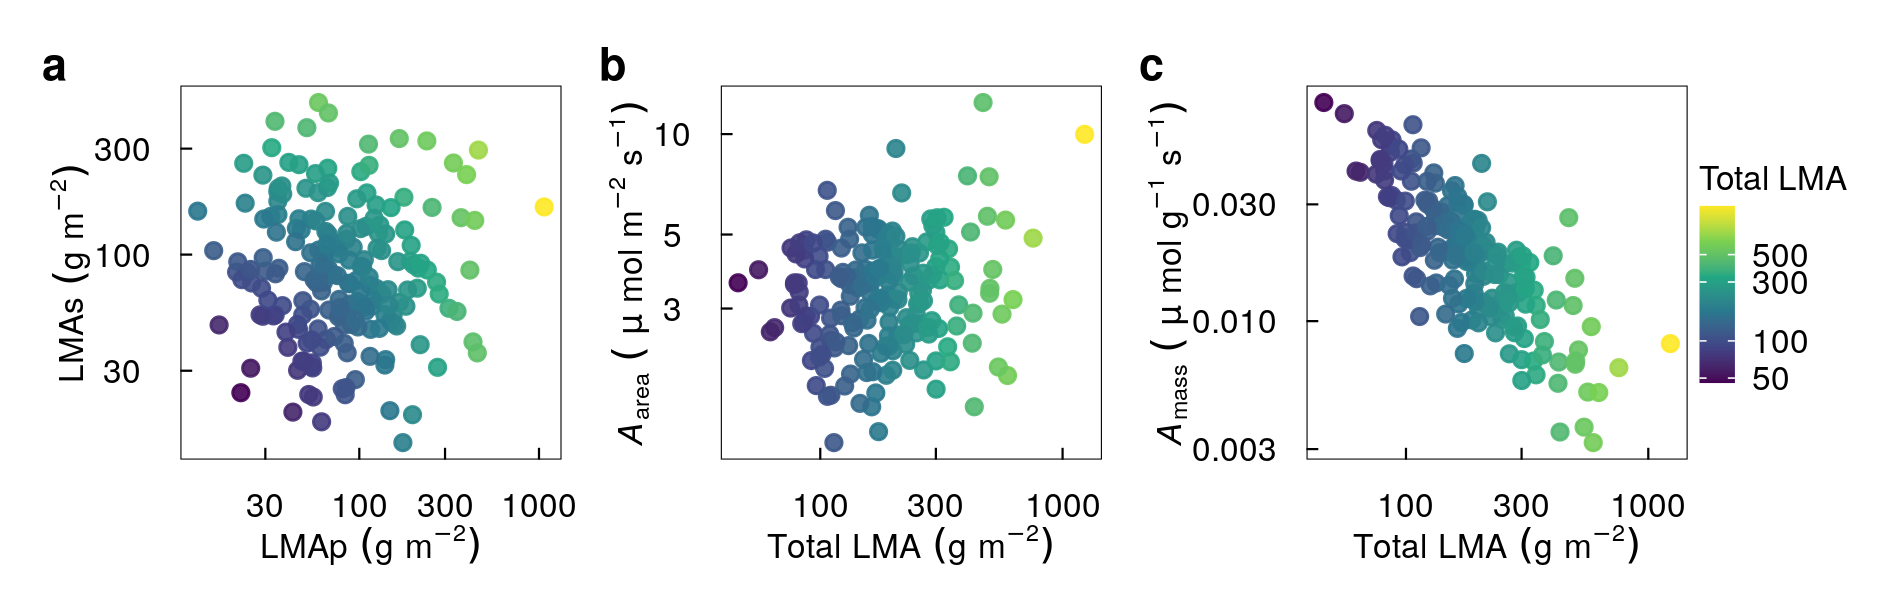
\includegraphics{/Users/mattocci/Dropbox/MS/LMAms/figs/hypo.png}

}

\caption{\label{fig-Hplt}Example of a two-dimensional functional space
that can result in either a two- or one-dimensional trait space,
depending on how metabolic traits are normalized. (A) Hypothetical
independent variation in two leaf mass per area (LMA) components:
metabolic leaf mass per area (LMAm, which largely determines per-area
values of photosynthesis, respiration, and nutrient concentrations) and
structural leaf mass per area (LMAs, which determines leaf toughness but
has little effect on metabolic traits). (B) Two-dimensional relationship
between photosynthetic capacity (\emph{A}) per-unit leaf area and total
LMA (equal to LMAm + LMAs). (C) One-dimensional relationship between
\emph{A} per-unit leaf mass and total LMA. LMAm and LMAs are simulated
from a hypothetical scenario of lognormal distributions with medians of
80 and standard deviations of exp(0.8) and exp(0.7), and zero
covariance. Variation in \emph{A} values are derived from our analysis
of the GLOPNET database.
\(A_{\mathrm{area} \, i}=1.77 \times \mathrm{LMAm}_i^{0.28}\mathrm{LMAs}^{-0.13}\epsilon_i\),
where \(\epsilon_i\) is log-normally distributed with log-mean with 0,
log-scale parameter with 0.31 (see Methods and Results).}

\end{figure}

\begin{figure}

{\centering 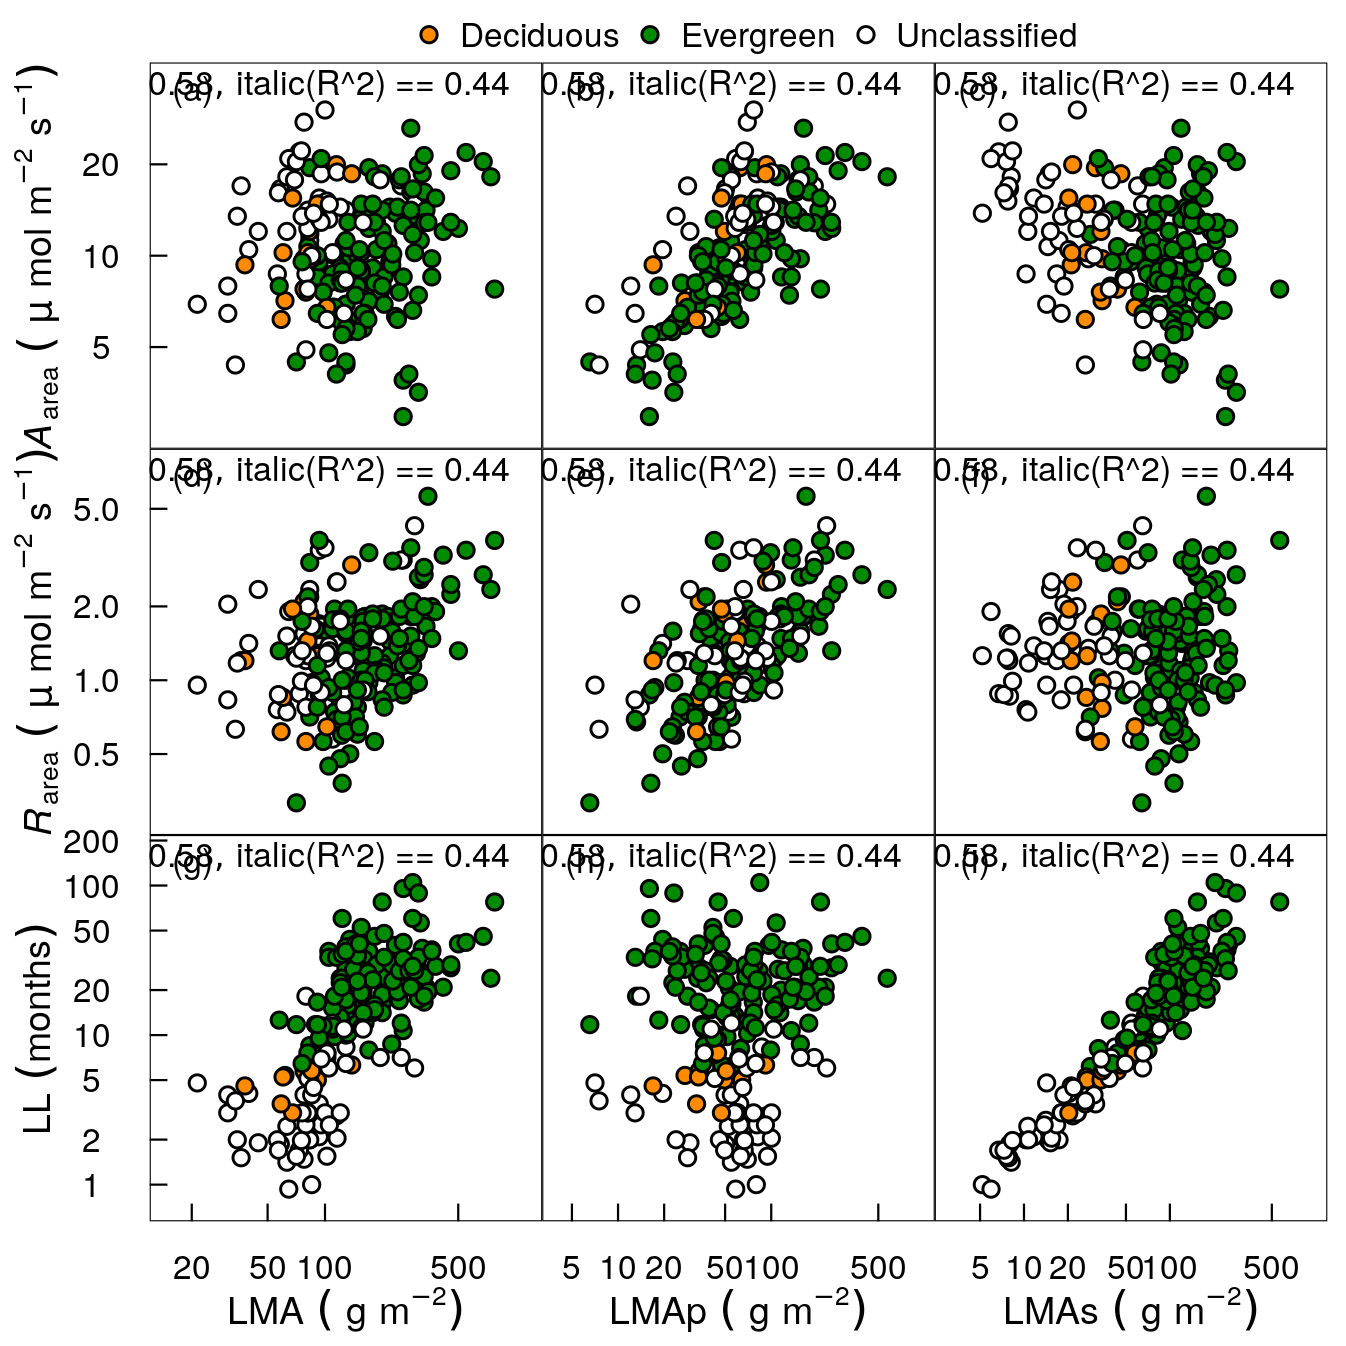
\includegraphics{/Users/mattocci/Dropbox/MS/LMAms/figs/gl_point.png}

}

\caption{\label{fig-GLplt}Observed and estimated leaf-trait
relationships in the global GLOPNET dataset. Estimates are from the best
GLOPNET model (Table 1). Leaf life span (LL), net photosynthetic rate
per unit leaf area (\emph{A}\textsubscript{area}), and dark respiration
rate per unit leaf area (\emph{R}\textsubscript{area}) are plotted
against observed LMA, posterior means of LMAm and LMAs. Pearson
correlation coefficients (\emph{r}) for LMA (left column) and posterior
means of Pearson correlation coefficients (\(\bar{r}\)) or partial
correlation coefficients (\(\bar{\rho}\)) for LMAm (middle column) and
LMAs (right column) are shown. Note that LL was modeled by LMAs alone
due to improved model performance with this parameter constraint (Table
1). Therefore, \emph{r} is reported for LL (single predictor variable),
whereas (\(\bar{\rho}\)) is reported for \emph{A}\textsubscript{area}
and \emph{R}\textsubscript{area} (multiple predictor variables).}

\end{figure}

\newpage

\begin{figure}

{\centering 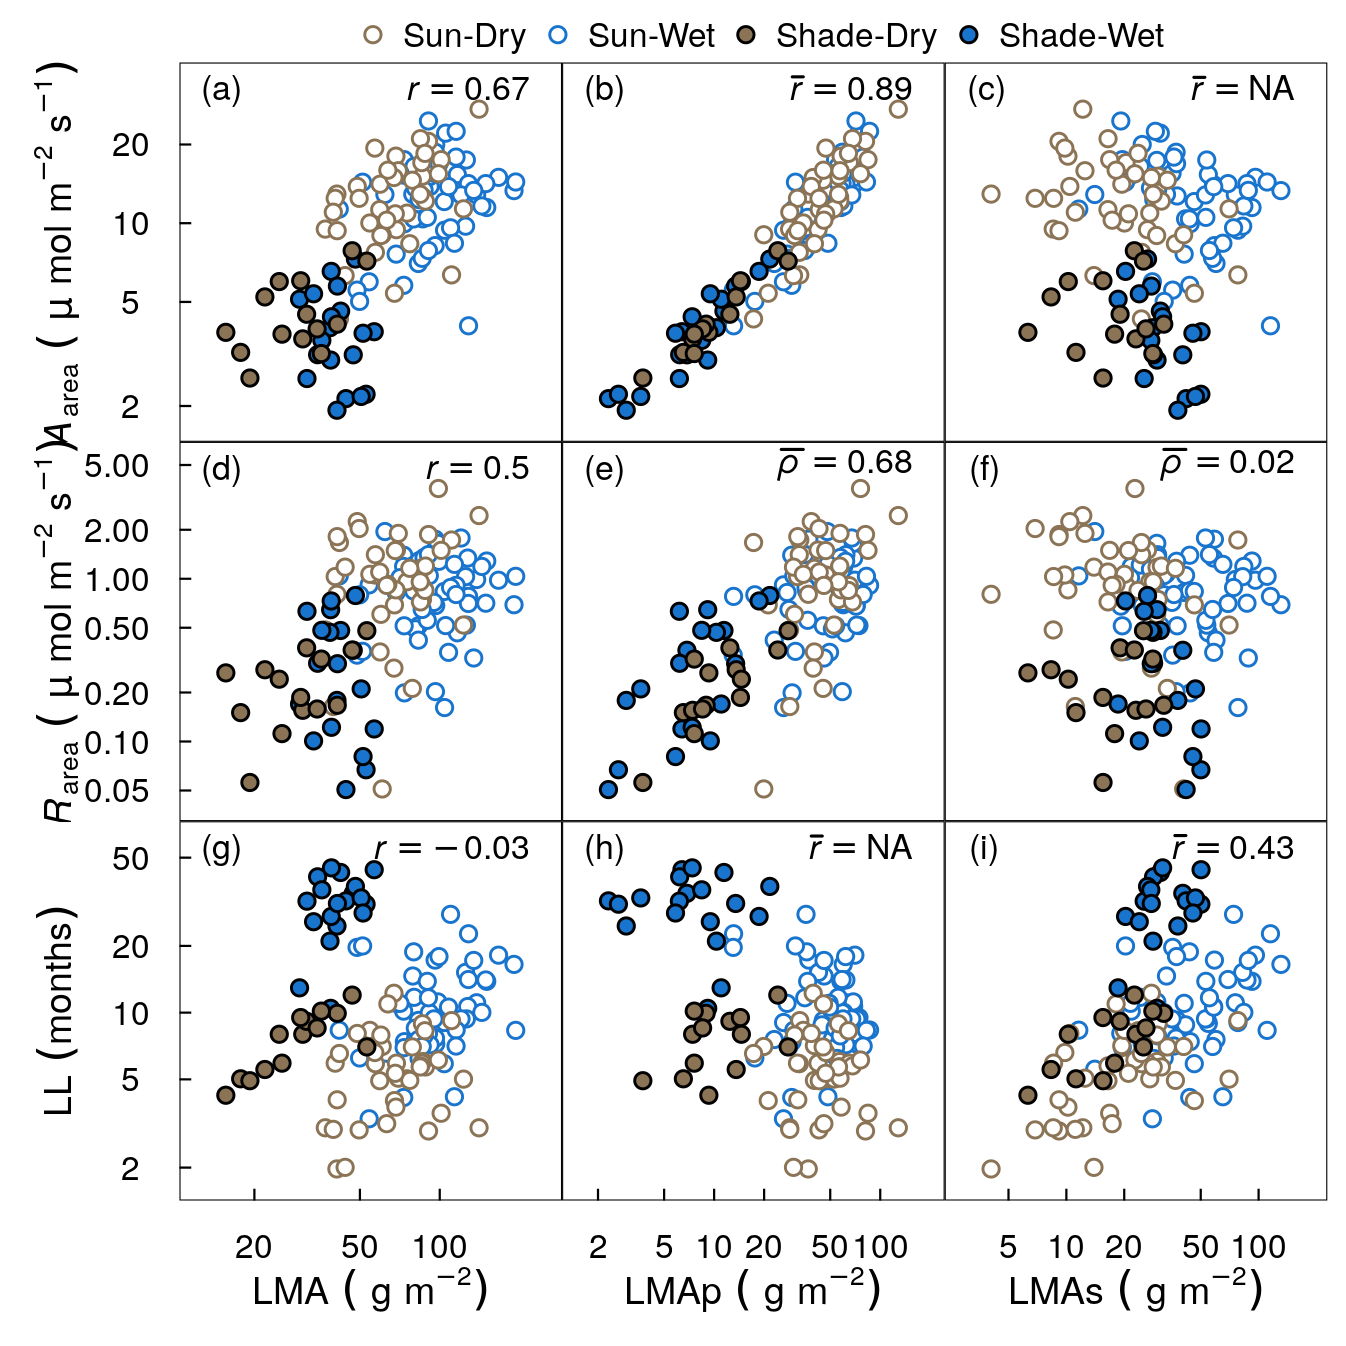
\includegraphics{/Users/mattocci/Dropbox/MS/LMAms/figs/pa_point.png}

}

\caption{\label{fig-PAplt}Observed and estimated leaf-trait
relationships in the Panama dataset. Estimates are from the best Panama
model (Table 1), which included effects of light on LL. Details as for
Fig.~\ref{fig-GLplt}. Results for other LL models are summarized in
Table SX. Note that \emph{A}\textsubscript{area} and LL were modeled by
LMAp and LMAs alone, respectively, due to improved model performance
with these parameter constraints (Table 1). The results shown here
include all leaves in the Panama dataset. The observed separation of LL
between sun and shade leaves is accounted for in the model predictions
Fig.~\ref{fig-LLplt}.}

\end{figure}

\newpage

\begin{figure}

{\centering \includegraphics{/Users/mattocci/Dropbox/MS/LMAms/figs/pa_point_par_ll.png}

}

\caption{\label{fig-LLplt}Relationship between leaf lifespan (LL) and
LMAs in the Panama dataset, afeter accounting for the effects of light
(suv vs.~shade leaves; see Eq. \ref{eq:LL_opt}). The dashed line
indicates the 1:1 relationship expected for residuals on the log-scale.
The posterior means of the partial correlation coefficient
(\(\bar{\rho}\)) is shown. The results shown here include all leaves in
the Panama dataset.}

\end{figure}

\newpage

\begin{figure}

{\centering \includegraphics{/Users/mattocci/Dropbox/MS/LMAms/figs/vpart_intra.png}

}

\caption{\label{fig-vpart}Variance partitioning on LMA components
between and within leaf habits (evergreen vs.~deciuous) for the GLOPNET
dataset and the Panama dataset, and between and within sites (wet
vs.~dry) and light (sun vs.~shade) for the Panama dataset. To isolate
the effects of intraspecific variation, the Panama results shown here
only include species for which both sun and shade leaves were
available.}

\end{figure}

\newpage

\begin{figure}

{\centering \includegraphics{/Users/mattocci/Dropbox/MS/LMAms/figs/box_de.png}

}

\caption{\label{fig-boxplt_de}Boxplots comparing leaf mass per area
(LMA) and posterior medians of photosynthetic and structural LMA
components (LMAm and LMAs, respectively) across deciduous (D) and
evergreen (E) leaves in the GLOPNET dataset (a) and in the Panama
dataset (b). The center line in each box indicates the median, upper and
lower box edges indicate the interquartile range, whiskers show 1.5
times the interquartile range, and points are outliers. Groups sharing
the same letters are not significantly different (P \textgreater{} 0.05;
t-tests). The Panama results only include species for which both sun and
shade leaves were available. Qualitatively similar results were obtained
when all Panama species were included (Fig. S\ref{fig-box_inter}). Note
that the vertical axis is on a log\textsubscript{10} scale.}

\end{figure}

\newpage

\begin{figure}

{\centering \includegraphics{/Users/mattocci/Dropbox/MS/LMAms/figs/box_pa.png}

}

\caption{\label{fig-boxplt_pa}Boxplots comparing leaf mass per area
(LMA) and posterior medians of metabolic and structural LMA components
(LMAm and LMAs, respectively) across sites (wet and dry) and canopy
strata (sun and shade) in the Panama dataset. These results only include
species for which both sun and shade leaves were available.
Qualitatively similar results were obtained when all Panama species were
included (Fig. S\ref{fig-box_inter}). Details as for
Fig.~\ref{fig-boxplt_de}.}

\end{figure}

\newpage

\begin{figure}

{\centering 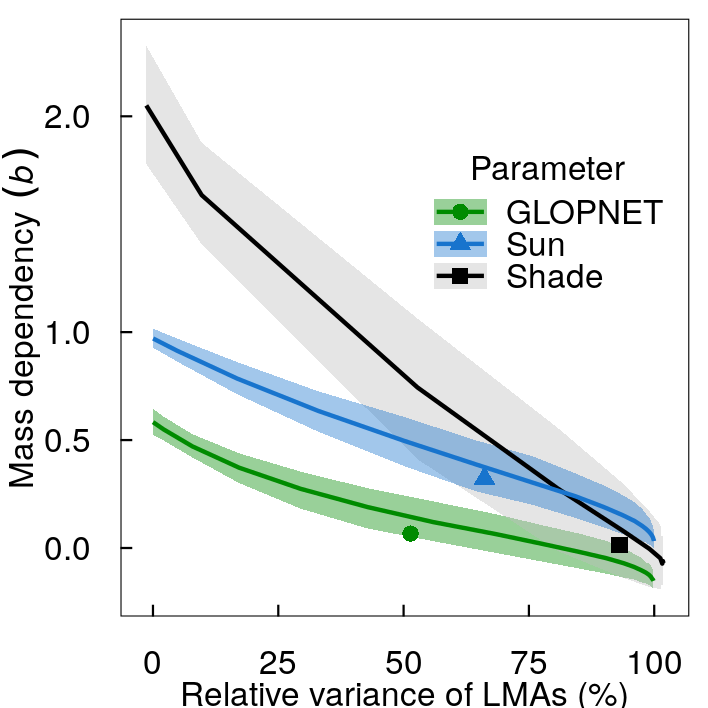
\includegraphics{/Users/mattocci/Dropbox/MS/LMAms/figs/mass_prop_mv.png}

}

\caption{\label{fig-massplt}Relationships between mass dependency
(\emph{b} in Eq.~\ref{eq-var}) and LMAs variance (relative to total LMA
variance) for the global GLPNET datase,t un leaves in Panama, and shade
leaves in Panama. Solid lines indicate simulated means and shaded
regions indicate 95\% CIs. Each point indicates the estimated values
from the empirical data and represents interspecific variation (e.g.,
across species within a canopy position in the Panama dataset). The
y-axis values indicates if photosynthetic capacity (\emph{A}) is is
primarily mass-dependent (\emph{b} \textgreater{} 0.5) or primarily
area-dependent (0.5 \textgreater{} \emph{b} \textgreater{} 0), with
\emph{b} near 0 indicating purely area-dependendence
(\protect\hyperlink{ref-Osnas2018}{Osnas et al., 2018}). If \emph{b}
\textgreater{} 1, then \emph{A} increases exponentially with LMA, which
is not consistent with observed relationships
(\protect\hyperlink{ref-Osnas2018}{Osnas et al., 2018}).}

\end{figure}

\newpage

\begin{figure}

{\centering 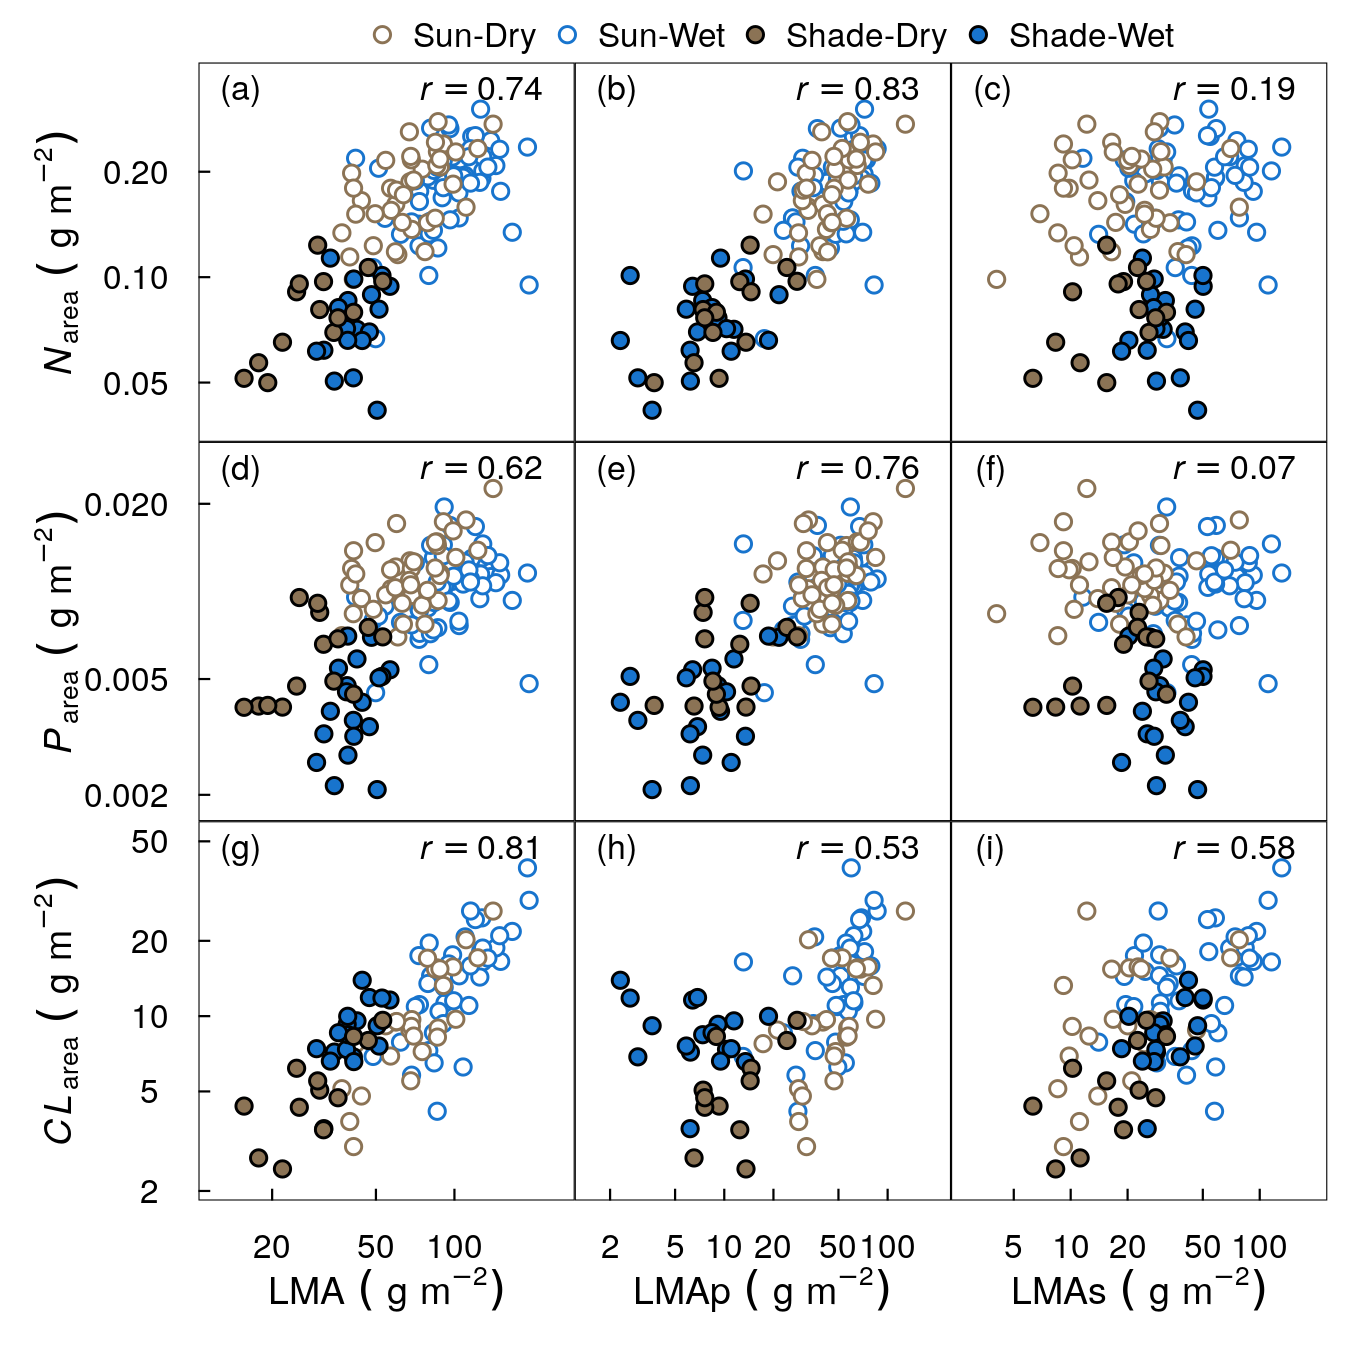
\includegraphics{/Users/mattocci/Dropbox/MS/LMAms/figs/pa_point_npc.png}

}

\caption{\label{fig-PA-NPC}Measured traits in the Panama dataset related
to photosynthesis and metabolism (nitrogen and phosphorus per-unit leaf
area; \emph{N}\textsubscript{area} and \emph{P}\textsubscript{area}) are
better correlated with estimates (posterior medians) of the metabolic
LMA component (LMAm) than the strctural component (LMAs), whereas the
opposite patten occurs for a measured structural trait (cellulose
per-unit leaf area; CL\textsubscript{area}).
\emph{N}\textsubscript{area}, \emph{P}\textsubscript{area}, and
CL\textsubscript{area} data were not used to fit the models, and are
presented here as independent support for the model results. Pearson
correlation coefficients (\emph{r}) for LMA (left column) and partial
correlation coefficients (\(\rho\)) of LMAm (middle column) and LMAs
(right column) are shown. Analogous results were obtained for
\emph{N}\textsubscript{area} and \emph{P}\textsubscript{area} for
GLOPNET (Fig. S\ref{fig-glnp}). The results shown here include all
leaves for which \emph{N}\textsubscript{area},
\emph{P}\textsubscript{area} and \emph{CL}\textsubscript{area} are
available.}

\end{figure}

\end{document}
